\chapter{Software and Simulation}
\label{ch:software}

\newcommand{\SimG}{\texttt{SimG4}\xspace}
\newcommand{\oaEvent}{\texttt{oaEvent}\xspace}
\newcommand{\Geant}{{\sc Geant4}\xspace}

% \begin{markdown}
% ---

% + Introduce ICEDUST, the COMET software suite
%     + Describe whole, then individual parts
%     + oaEvent
 
% + Important part of the software is the set of simulation tools
%     + COMET geometries
%     + Physics, "physics list"?
%     + Show signal event display
%     + SDs, CDC hit representation
%     + RooTracker files
%     + Proton beam input?
%     + Hit merging and bunch simulation
%     + Large-scale production, MC5: Sampling world, example of results?
    
    
% + Version control
% + Continuous integration (+ CD, docker containers)
    
% + Mention miscellanous contributions:
%     + Beginner's tutorial (installation, simulation, analysis)
%     + Move from CMT to CMake and from ROOT5 to ROOT6
%     + Memory leaks and errors
%     + Backward MC: perhaps just ref chapter

% + Animated visualisation of CyDet activity

% ---
% \end{markdown}

Experiments in high energy physics are commonly accompanied by the development
of a set of software tools to help in manipulating and analysing experimental
data. Simulations are used extensively to optimise experimental designs and
prepare for the collection of real data while the physical instruments ---
detectors, magnets, readout electronics and data acquisition systems --- are
being manufactured and assembled.

\section{The ICEDUST Software Suite}
The COMET Collaboration develops a suite of software packages named ICEDUST
(Integrated COMET Experimental Data User Software Toolkit) to satisfy the
offline data-processing requirements of the experiment. Originally forked in
2013 from the software written for T2K's near detector system ND280, ICEDUST
supports the needs of the COMET experiment with regard to simulation, on-disk
data format, calibration, reconstruction and analysis.
Figure~\ref{fig:icedust_schematic} shows the flow of real and simulated data
within the ICEDUST framework, and lists the names of the key packages for each
step.


\begin{figure}
    \centering
    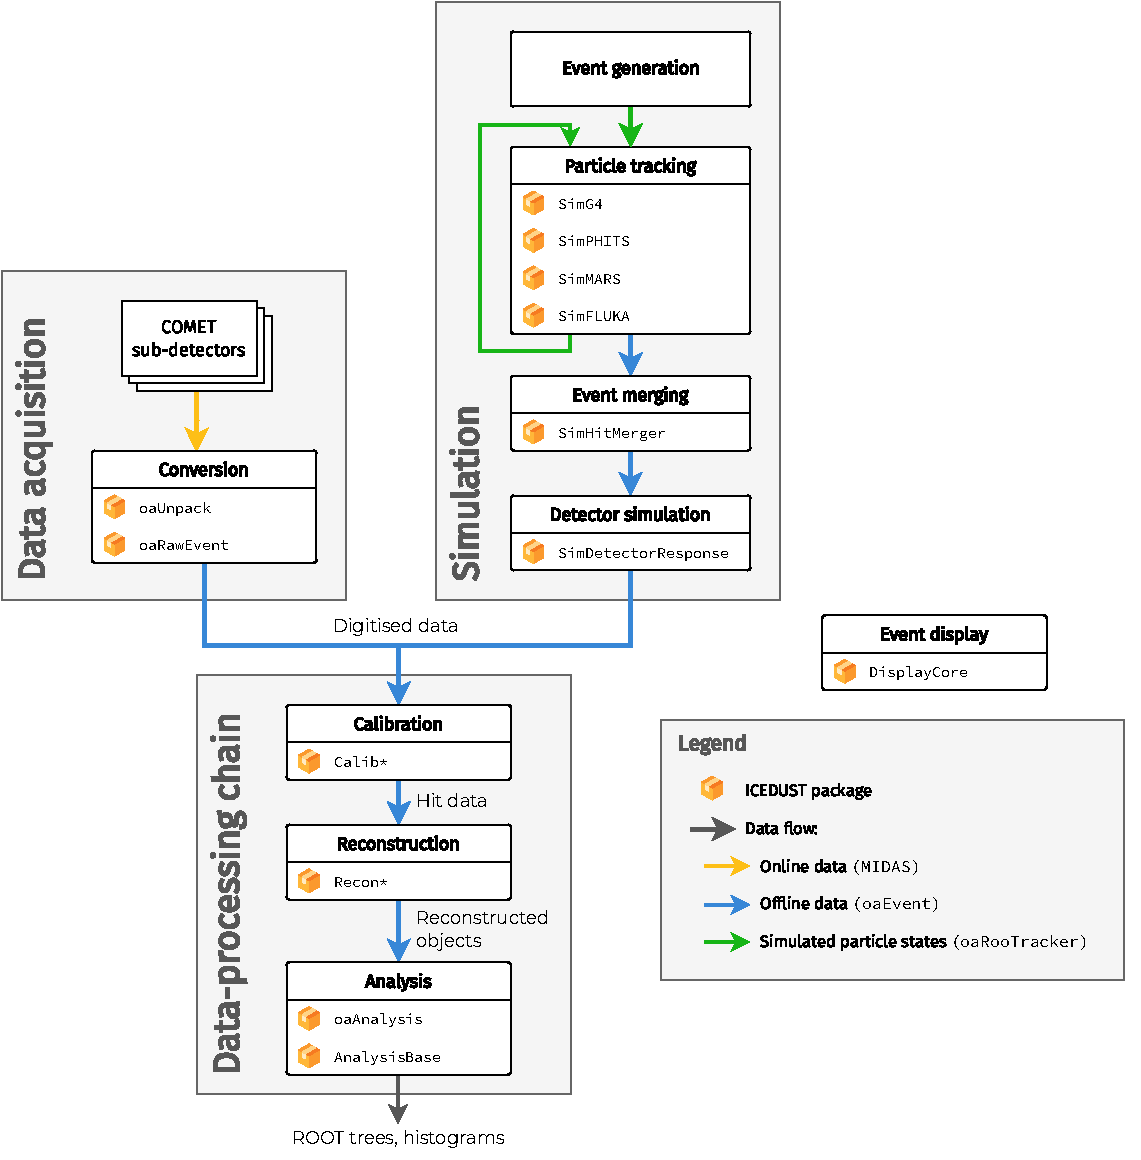
\includegraphics[width=0.9\textwidth]{chapter3/ICEDUST_vertical.drawio.pdf}
    \caption{Data flow in the ICEDUST framework. The colour of arrows represents
        the data format. By design, simulated detector data and real data share
        a common format such that they can be processed identically by the
        calibration, reconstruction and analysis stages.}
    \label{fig:icedust_schematic}
    \vspace{1.2cm}
    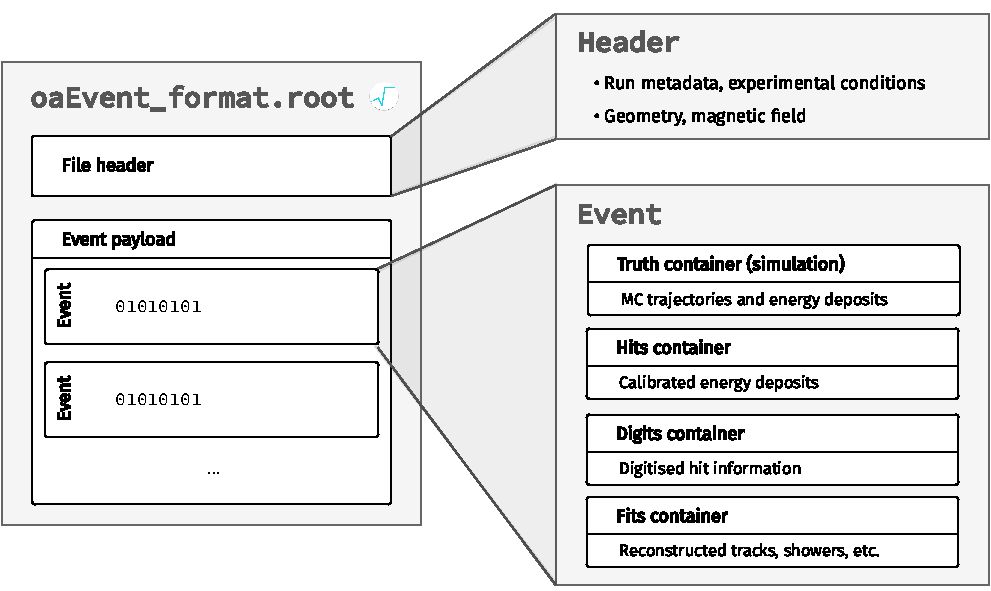
\includegraphics[width=0.6\textwidth]{chapter3/oaEvent.drawio.pdf}
    \caption{Layout of \oaEvent files which contain MC or real data. Blue arrows
    in Figure~\ref{fig:icedust_schematic} indicate steps of the data flow where
    data is stored in this format on disk.}
    \label{fig:oaEvent}
\end{figure}

\subsection{Data format}
A key design principle of ICEDUST is to define a common format adopted by both real and simulated data, such that the pipeline of calibration, reconstruction and analysis can be thoroughly tested with only simulation data, in advance of the data acquisition stage. 
This offline data format is called \oaEvent. Based on the ROOT~\cite{BRUN199781} serialisation system, \oaEvent defines a file format where data is laid out as a sequence of events, shown schematically in Figure~\ref{fig:oaEvent}. Each event object contains an arborescence of data containers, each of which holds an array of some given data type (e.g.\ detector hits, calibrated energy deposits, reconstructed tracks, etc.).

From Phase-I onward, data will be collected using the MIDAS data acquisition system, hence the online on-disk format is based on MIDAS data banks. ICEDUST provides a direct translation from this format to \oaEvent via the \texttt{oaRawEvent} and \texttt{oaUnpack} packages. Once translated, the data can flow through the calibration, reconstruction and analysis stages.

%Prior to calibration, the resulting data will typically represent uncalibrated, digitised detector hits or waveforms. 

%The term ``event'' here is purposefully abstract, as the information held in each event can vary. In simulations, an event can describe the outcome of a single proton-on-target (POT) collision, or the outcome of a full proton bunch ($16\times10^6$ POT). 
%In data-taking runs, the definition of event will typically be dictated by the data acquisition system.  % So?



%Each event is its own hierarchical ``directory'', where data containers can be stored and retrieved by name. The containers themselves are variable-length arrays of arbitrary data types---defined as C++ classes---where objects of the same type can be aggregated.


%The calibration step uses pre-established calibration databases for each sub-detector to convert the digitised information into physical information such as the energy deposit and time that constitute hits. The reconstruction algorithms process hits to find tracks and filter out background, to pass that information down to the final analysis stage.

\subsection{Simulation pipeline}
Simulations of the COMET experiment can be split into four steps:
\begin{enumerate}
    \item {\bf Event generation} takes place at the level of individual protons. A proton beam profile is drawn ahead of time using a specialised Turtle~\cite{Carey1974DecayT} simulation of the beamline. The position and momentum of the protons are histogrammed at a short distance ahead of the pion-production target. Protons are sampled from the resulting distribution to generate events, and the outcome from each primary proton is referred to as a proton-on-target (POT) event.
    \item {\bf Particle tracking} is the step-by-step propagation of particles through the geometry and electromagnetic fields of the experimental setup. The primary proton will usually produce many secondary particles in the collision, some of which might propagate to the detector region. Simulated energy deposits in the active detector volumes are recorded for the detector response simulation stage.
    \item {\bf Event bunching} allows us to model the simultaneous arrival of a proton bunch into the setup. In the real beamline, millions of protons are bunched into a short \SI{{\sim} 100}{\ns} time interval, and two consecutive bunches are separated by about \SI{1.2}{\micro\second}. In order to simulate this time structure, a time offset is applied to each POT event, after which the events are merged into bunches. Following this, individual bunch events can be further merged into \emph{bunch trains} to obtain an entire sequence and account for potential pileup.
    \item {\bf Detector response simulation} translates the true energy deposits simulated in the particle tracking stage into detector-specific hits. It takes into account the way in which charge or light is collected by the detector, and can apply smearing to the observed energy and timing. This step effectively reverses the calibration process by transforming energy deposits into uncalibrated, digitised hits and waveforms.
\end{enumerate}
% ^ OK
Once all four stages of the simulation pipeline are complete, the result should closely resemble real data post-translation from MIDAS to \oaEvent. This implies that it should be able to naturally flow through the calibration, reconstruction and analysis stages. At each stage, the information may be compared with the truth information available from the particle tracking stage in order to refine each process. This exercise should also outline the performance of the offline data-processing pipeline and hence provide an estimate of the computational requirements of the experiment.


\subsection{Intermediate simulation file format}
\label{subsec:RT}
The \texttt{oaRooTracker} package defines another ROOT-based file format used by the simulation to save and retrieve particle states. The typical use case is for a simulation to record particles that have reached a key geometrical element (e.g.\ the detector region) to build up a sample of interesting events. The saved particle states can then be used as input to subsequent simulations, easing the need for a full simulation run every time a change is made to the geometry or physics models.

In addition, from a large enough sample of particles recorded at some key volume boundary, the flux distribution of inbound particles can be estimated. Events can then be sampled from this distribution to increase the statistics inside the volume of interest. 

% RooTracker files
%The simulation software provides utility to record particles that reach certain key points in the geometry, such as the transport solenoid or the detector region. Virtual monitors are volumes that can be placed in the geometry to record the passage of particles, in the form of virtual hits or into a separate file. The file format used to save particle states is called \texttt{RooTracker}. It stores the kinematics of simulated particles and can thus be used as input to another simulation run. % and?

\section{Monte Carlo simulation in ICEDUST}
\label{sec:mc_sim}
Monte Carlo (MC) simulation is the process through which hypothetical particles are realistically propagated through an experimental setup, with the aim of evaluating the experiment's performance and to prepare for its realisation. Currently in COMET, MC simulations are heavily used to further optimise the experiment's design and to develop reconstruction and analysis algorithms.

Monte Carlo simulation in high energy physics can be described as the stepwise propagation (tracking) of particles through matter and electromagnetic fields. Starting from initial conditions of position and momentum, a particle advances in space and time according to the laws of relativistic kinematics. It can change velocity or direction, and produce secondary particles via interactions with the local medium and field. The tracking of a particle ends when it decays, gets absorbed by some material, or exits the simulation space.

Interactions and decays occur stochastically according to measured cross-sections and lifetimes. Depending on the type of interaction, secondary particles may be emitted. In this case, the position and momentum of secondaries are stored in memory until the tracking of the primary particle is finished. The list of secondaries is then iterated through, propagating each one in turn. Since secondaries may produce their own secondaries, this process continues recursively until all products of the original primary particle have been accounted for.
% ^OK

In ICEDUST, particle tracking, event bunching and detector response simulation are handled in separate packages.
Particle tracking can be performed using four different engines: Geant4~\cite{AGOSTINELLI2003250}, FLUKA~\cite{FLUKA}, MARS15~\cite{MARS15} and PHITS~\cite{PHITS}. The corresponding ICEDUST packages are \SimG, \texttt{SimFLUKA}, \texttt{SimMARS}, and \texttt{SimPHITS}, respectively.
Event bunching is handled by the \texttt{SimHitMerger} package, and \texttt{SimDetectorResponse} performs detector response simulation.

\subsection{Geometry}
The \SimG package contains the most detailed and up-to-date definitions of the COMET simulation geometries.
The various components that make up a simulation world are defined with constructive solid geometry, using the standard \Geant geometry classes. In addition, \SimG extends the \Geant macro language to allow geometrical parameters to be defined in macro files. The position, dimensions, and material of every volume can thus be specified at run-time rather than compile-time. A custom parser attached to every volume allows interdependencies between components and supports looping, for instance to position identical elements in a regular pattern.

Once the simulation geometry is assembled, it is also translated into the ROOT \texttt{TGeo} representation, which simplifies its visualisation and its storage on disk as metadata inside \oaEvent files. This representation can furthermore be interpreted by the MARS15 tracking software, which simplifies the process of running comparative simulations.

%Once the whole geometry is assembled, it is translated into an equivalent ROOT representation that will be stored into the output file for book-keeping. This copy can also be rendered more readily by the 3D utility classes of the ROOT package. % Link to DisplayCore? !! REMOVED --> out of scope of section?


The \SimG package includes geometries for the Phase-$\alpha$, Phase-I (CyDet and StrawECAL configurations), and Phase-II setups. Over time, these simulation worlds are refined by developers to better reflect the exact configuration of the experiment. 
Figure~\ref{fig:comet_geometries} shows the simulation geometries for the two conversion-searching COMET designs.

\begin{figure}
    \centering
    \captionsetup[subfigure]{justification=centering}
    % To make this figure: thin wireframes, white background
    % Plane clipping at y=10
    % zoom all the way out and move the camera forward (right-click)
    % so the perspective approaches an isometric view.
    \noindent\makebox[\linewidth][c]{
    \begin{subfigure}[t]{0.57\textwidth}
        \centering
        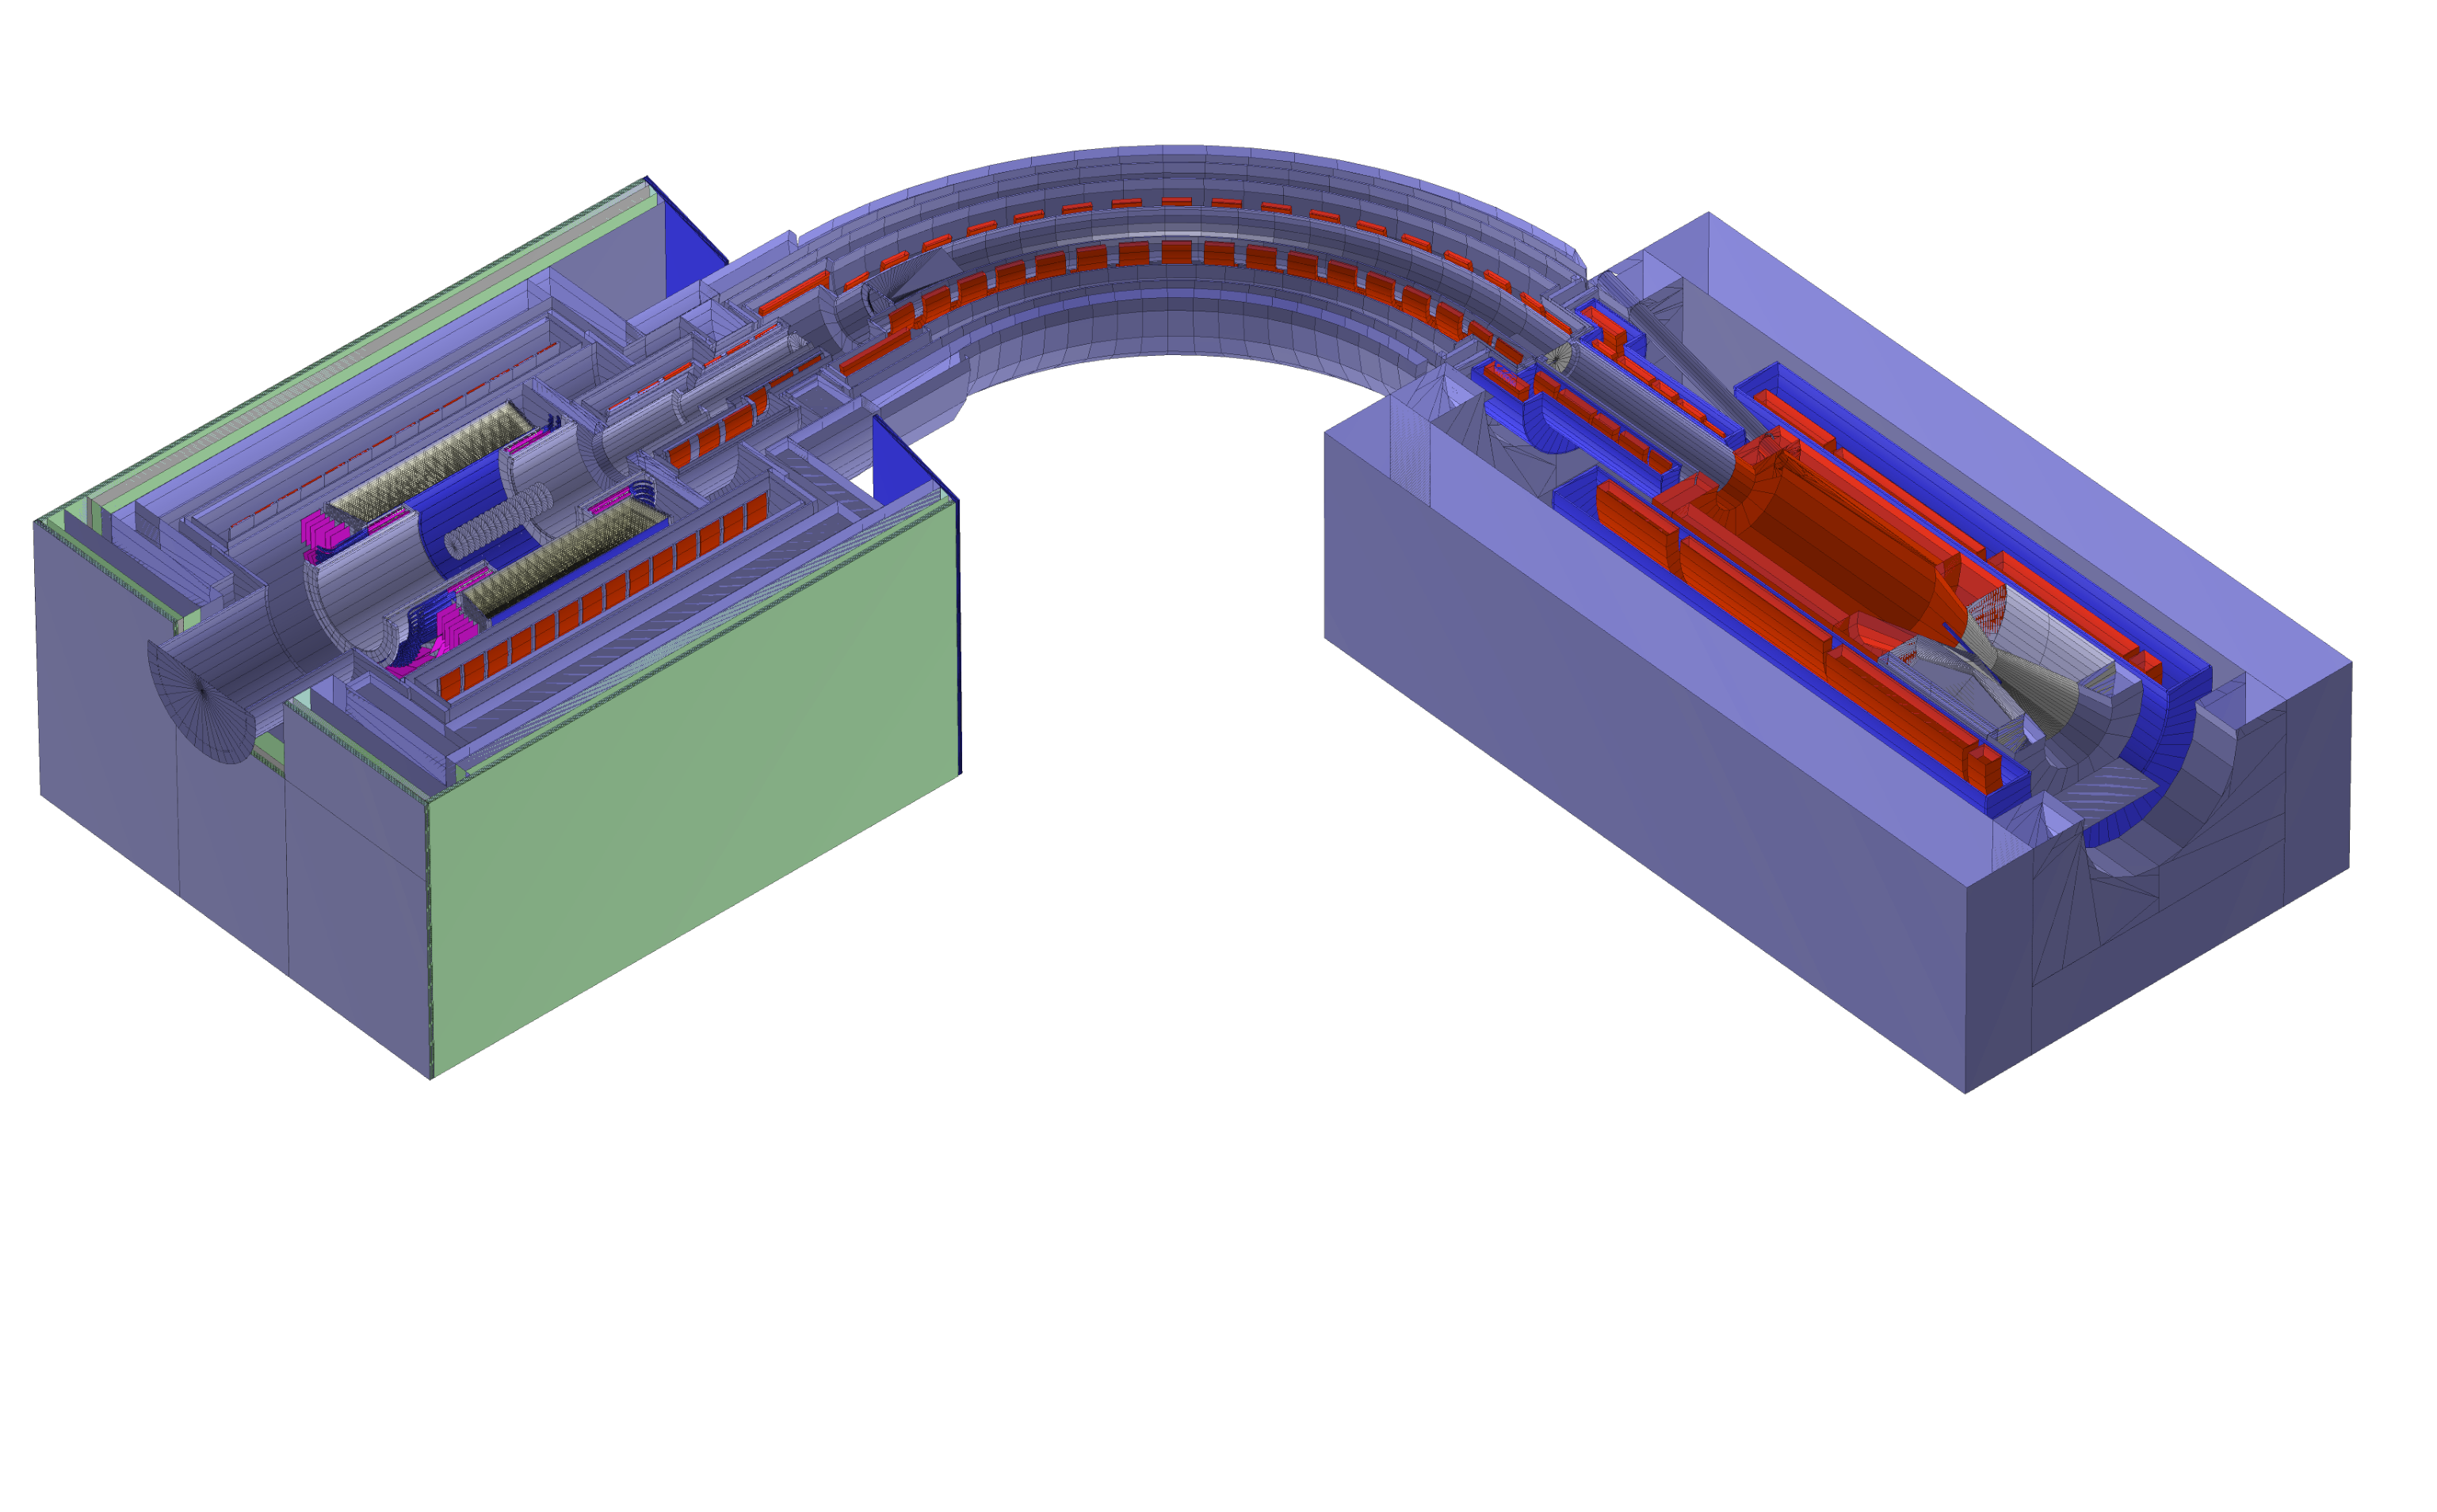
\includegraphics[width=0.95\textwidth]{chapter3/geometries_Phase-I_iso_cropless_huesat_croppedleft.png}
        \caption{Phase-I in the CyDet configuration.}
    \end{subfigure}
    \hfill
    \begin{subfigure}[t]{0.57\textwidth}
        \centering
        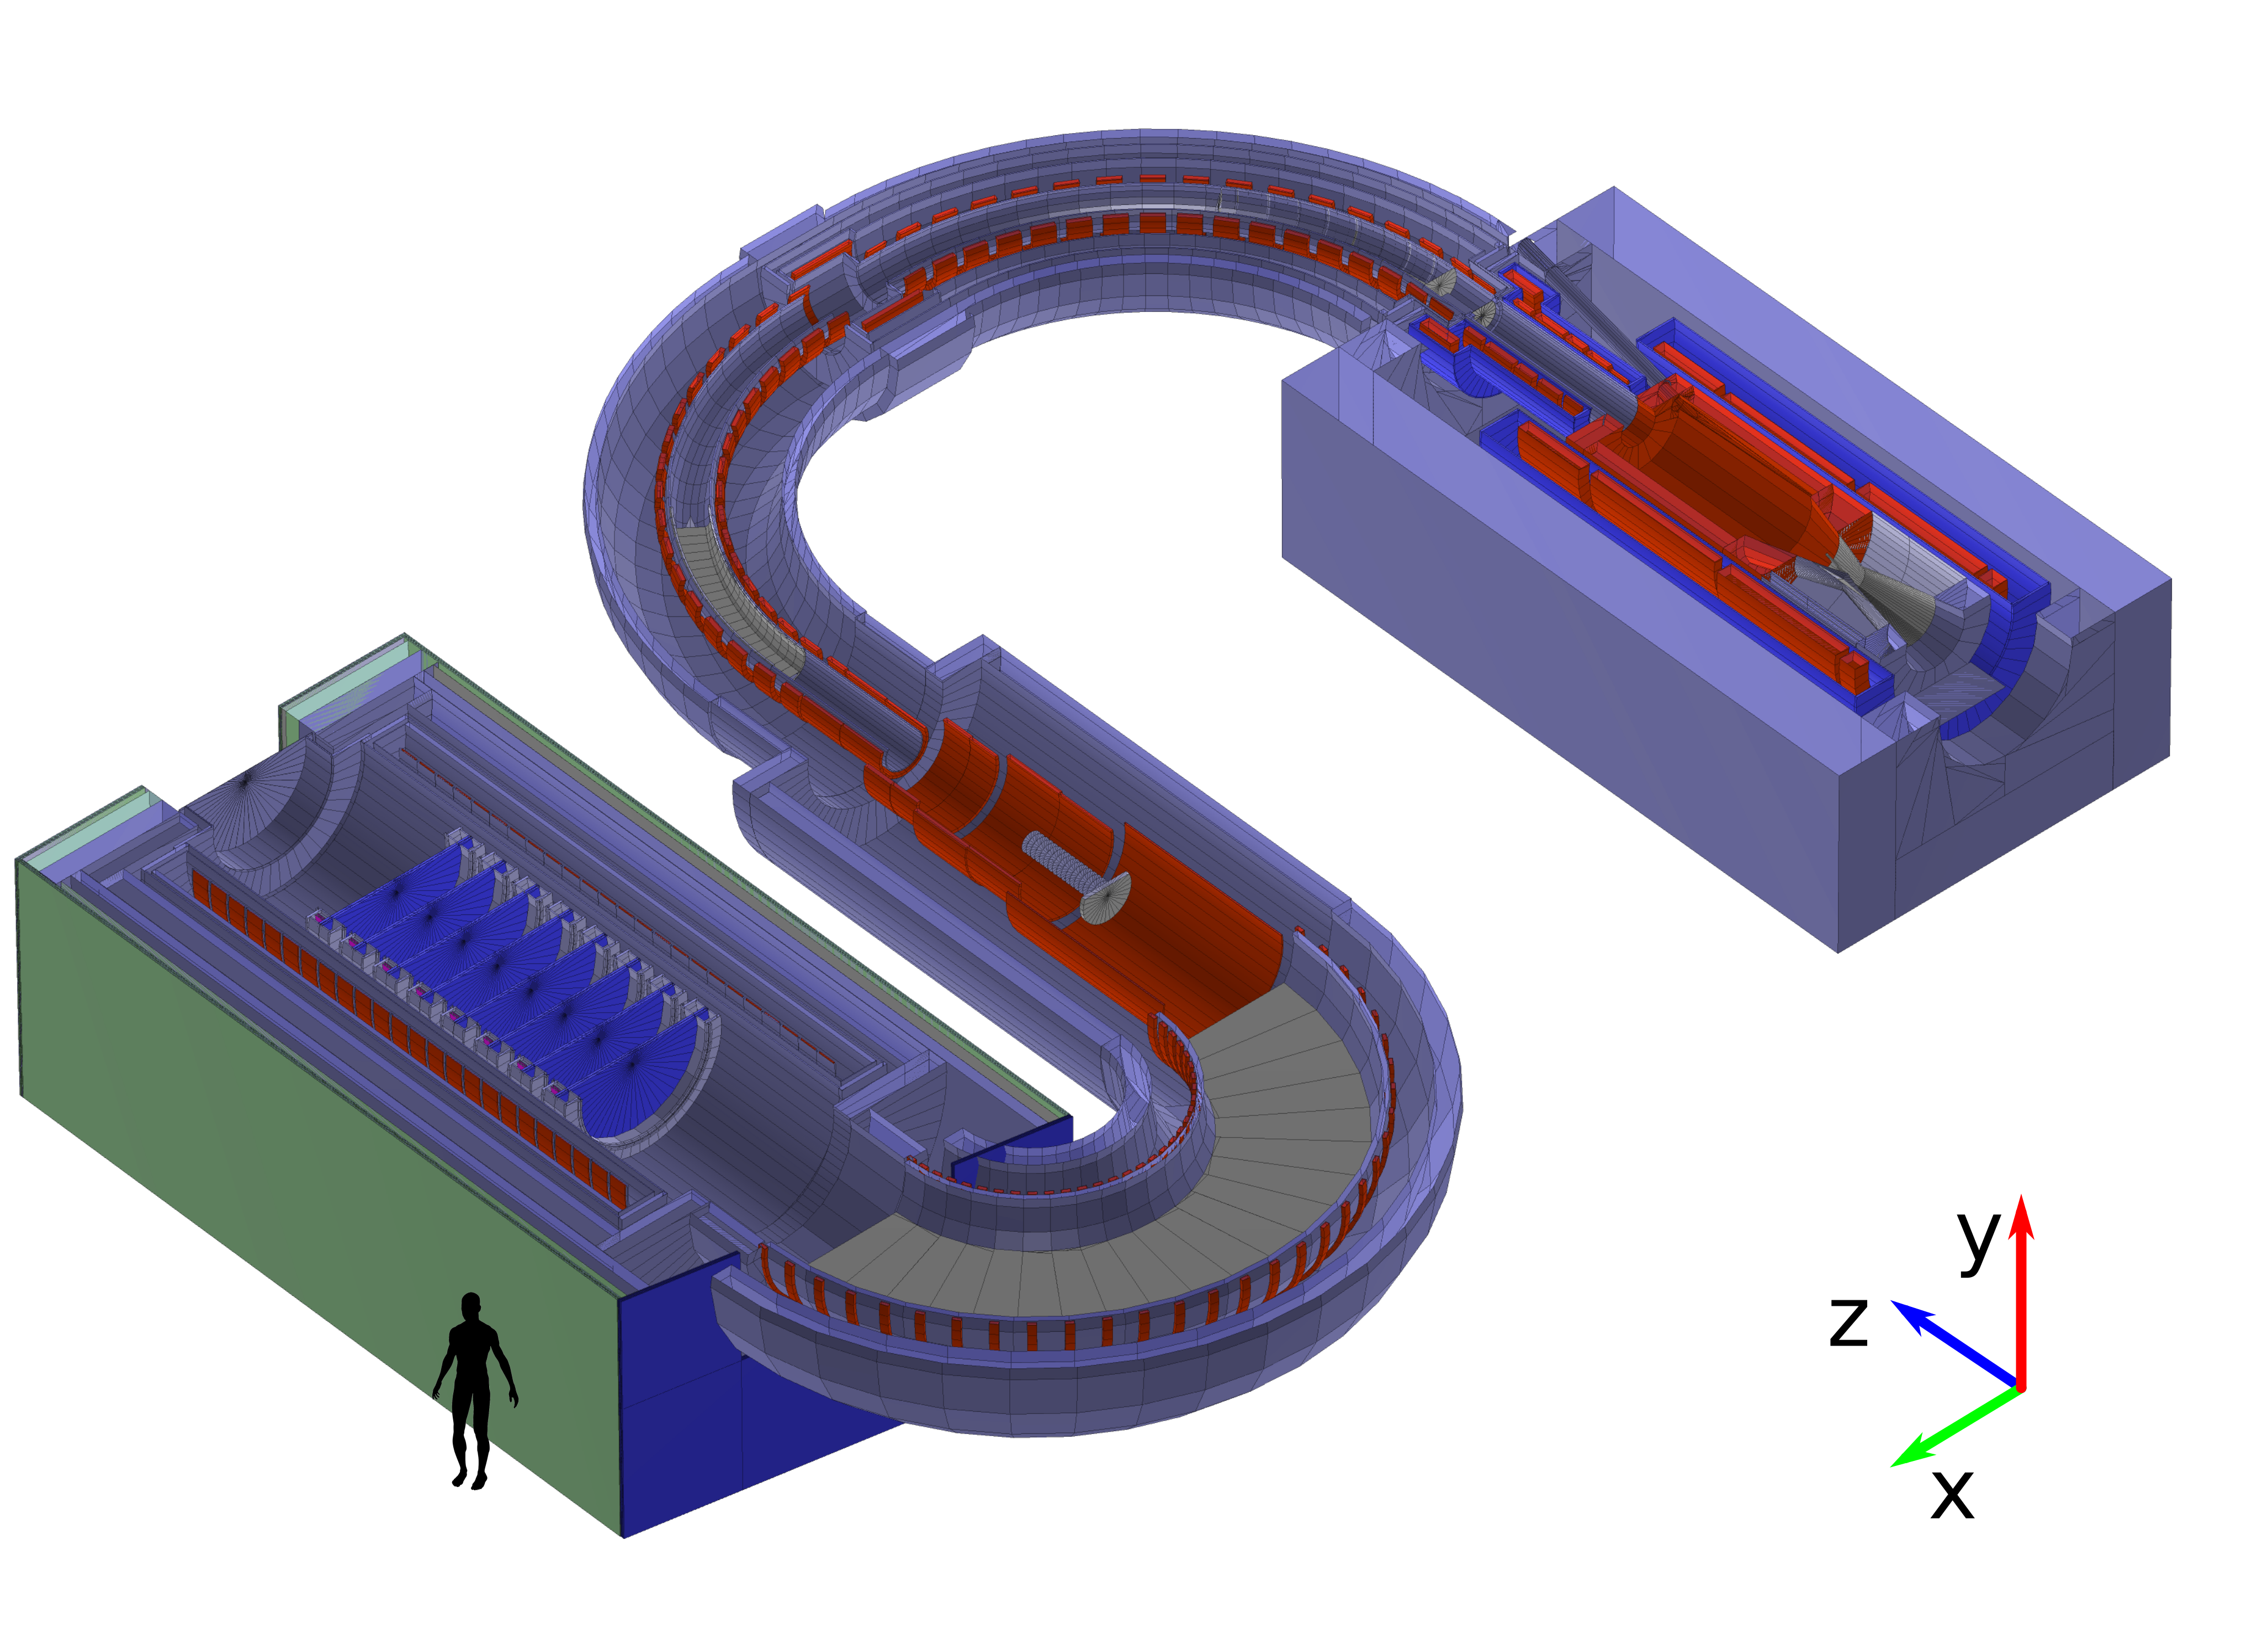
\includegraphics[width=0.95\textwidth]{chapter3/geometries_Phase-II_iso_huesat_human.png}
        \caption{Phase-II.}
    \end{subfigure}}
    
    \caption{Cutaway views of the simulation geometries implemented in \SimG and visualised with \texttt{DisplayCore}. The experiment hall is also modelled in the simulation but was hidden here for clarity.}
    \label{fig:comet_geometries}
\end{figure}

% vvvv Moved to first section
% % Event generation 
% \section{Event generation and bunch structure}
% Protons are sampled from a beam profile histogram at a distance of \SI{70}{\cm} upstream of the target. The histogram is generated via a Turtle~\cite{Carey1974DecayT} simulation of the proton beamline.

% In the simulation, a single proton is sampled from the beam histogram for each event, which differs from the real situation in that the actual beam is arranged into bunches, each containing about 16 million protons. Hence we assume that proton collisions in a bunch are independent of each other, and we merge POT events into bunch events by overlaying the produced trajectories and hits. This task is handled by the \texttt{SimHitMerger} program after \SimG has finished simulating single-proton events. The time structure of the proton bunch is modelled as a square wave with a width of \SI{100}{\ns}. To simulate this structure, a time shift is sampled uniformly between -50 and \SI{50}{\ns} for each POT event and applied to every trajectory and hit.

% \hl{Refer to, or show a time structure diagram}
% ----------

\subsection{Physics}
The COMET experiment involves many physical processes to go from the initial proton collision to backgrounds in the detector.
The MC simulation must faithfully account for any process which could lead to backgrounds if we are to realistically estimate the experiment's sensitivity. 
Hence, the \SimG simulation associates standard \Geant hadronic and electromagnetic physics lists with custom logic for nuclear muon capture and muon decay-in-orbit.

To model hadronic interactions, \SimG uses the \texttt{QGSP\_BERT\_HP} reference physics list as the default. In this model, hadron-nucleus interactions between the \SI{8}{\GeV} proton beam and the pion-production target are handled by the Bertini Cascade model~\cite{WRIGHT2015175}.

Muons at rest receive special treatment in \SimG due to their important
contribution toward the background rate. The default energy spectrum of
electrons from muon decay-in-orbit is replaced by the numerical evaluation
of~\cite{czarnecki}, which includes the effect of nuclear recoil and thus allows
electron energies up to \SI{104.973}{\MeV}. In addition, the nuclear muon
capture (NMC) model is replaced to adhere to the results of the AlCap
experiment~\cite{PhysRevC.105.035501} which measured the energy spectrum of
protons emitted after NMC in aluminium.




\subsection{Signal simulation}
By default, the list of physical processes considered by \SimG includes only
SM-allowed interactions and decays, and hence does not include $\mu$--$e$
conversion. In order to simulate signal events, one can manually produce
conversion electrons out of the muons stopped inside the stopping target.

From the normal beam simulation, one can estimate the spatial and temporal
distributions of muons being stopped in the stopping target, and subsequently
sample conversion electrons from it. In sensitivity studies, signal events are
commonly overlaid onto a pure background sample in order to evaluate the signal
acceptance and background rejection efficiencies of the hit filtering and track
finding routines. % Accurate?

%% Moved to COMET chapter
% \begin{figure}
%     \centering
%     \captionsetup[subfigure]{justification=centering}
%     \begin{subfigure}[t]{0.43\textwidth}
%     \centering
%     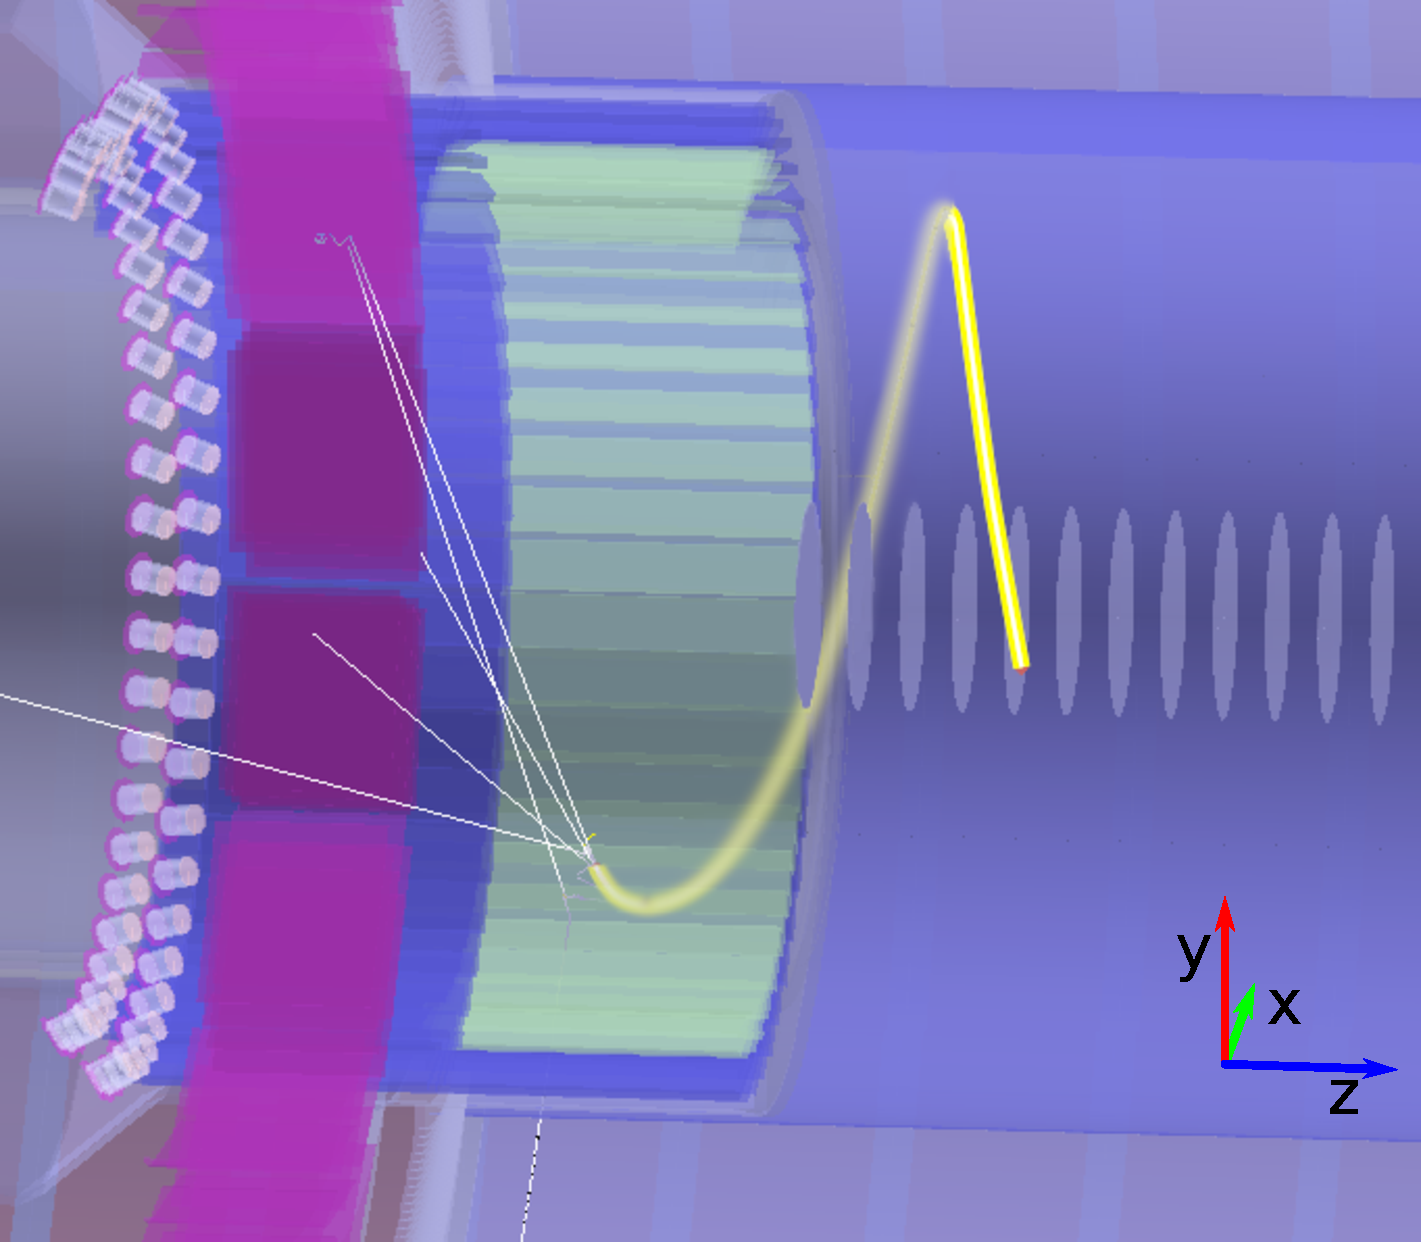
\includegraphics[width=0.95\textwidth]{chapter3/signal_event_display_crop_axes.pdf}
%     \caption{Event shown in \texttt{DisplayCore}, the 3D event display.}
%     \end{subfigure}
%     \hfill
%     \begin{subfigure}[t]{0.48\textwidth}
%     \centering
%     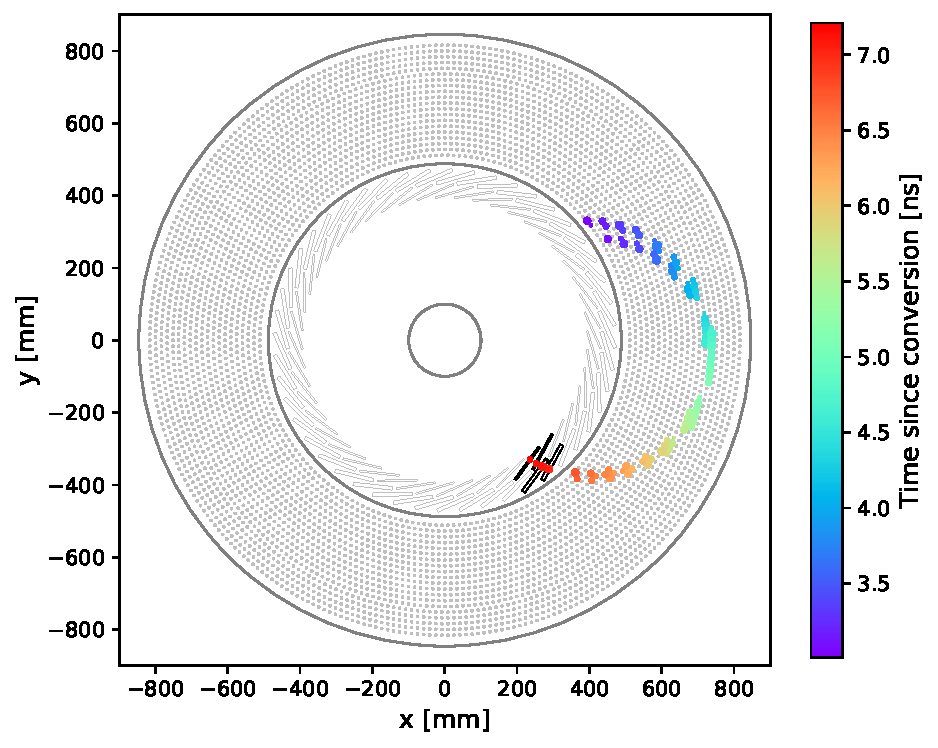
\includegraphics[width=0.95\textwidth]{chapter3/cydet_signal_track_v2.pdf}
%     \caption{Event as seen by the CDC and CTH detectors.}
%     \end{subfigure}
    
%     \caption{Example of a simulated signal trajectory in the CyDet system. This particular event triggers the CTH and would be considered as an ideal candidate of a $\mu$--$e$ conversion signal.}
%     \label{fig:signal_event}
% \end{figure}

Figure~\ref{fig:cydet_signal_event} shows a simulated conversion electron
emerging from the stopping target, depositing energy inside the CDC gas, to
eventually trigger the CTH by hitting four adjacent counters. 

\subsection{Representation of simulated CDC hits}
\label{subsec:SD}
% Sensitive detectors, truth-hit representation
As a particle passes through a material, it tends to lose energy to the medium, e.g. through inelastic scattering or ionisation. 
In MC simulations, simulated energy deposits must be recorded inside active detector elements in order for us to determine the response of the detector and readout systems to the passage of the particle.

Detector elements in a \Geant simulation are defined as ``sensitive volumes'', and energy deposits of incoming particles are accumulated and recorded as ``hits''. 
The way in which hits are instantiated is typically dependent on the type of detector, because of differing granularities between e.g.\ a plastic scintillator and a drift chamber. A higher-granularity detector type requires finer-detailed information, hence more hit instances along the trajectory.

In \SimG, the data type associated with CDC hits is called \texttt{IG4HitGas}. When \Geant reports an energy deposit inside the CDC, an instance of that class is created. If a particle makes multiple steps in a CDC cell, the deposit from each step is accumulated into the same hit instance, such that only one instance per particle per cell may exist. If a particle enters the same cell multiple times, one hit instance is created per entry.
This is shown in Figure~\ref{fig:sim_cdc_hits}, where the position and granularity of \texttt{IG4HitGas} instances is drawn along an electron's trajectory in the CDC.


% In early 2019, ICEDUST developers agreed to change the definition of hits inside the CDC gas volume in order to more accurately portray the energy deposit information in that detector. Along that process, I came to be thoroughly involved in the testing and refinement of this new CDC hit representation, named \texttt{IG4HitGas}. 

% A hit representation is formulated as a C++ class which holds the hit's data. It must be coupled to a sensitive detector class, whose role is to receive information from \Geant's particle tracking system and accumulate it into instances of the hit class. For example, the sensitive detector class for a calorimeter might produce hits containing the total energy deposited for each inbound particle as well as a timestamp.

\begin{figure}
    \centering
    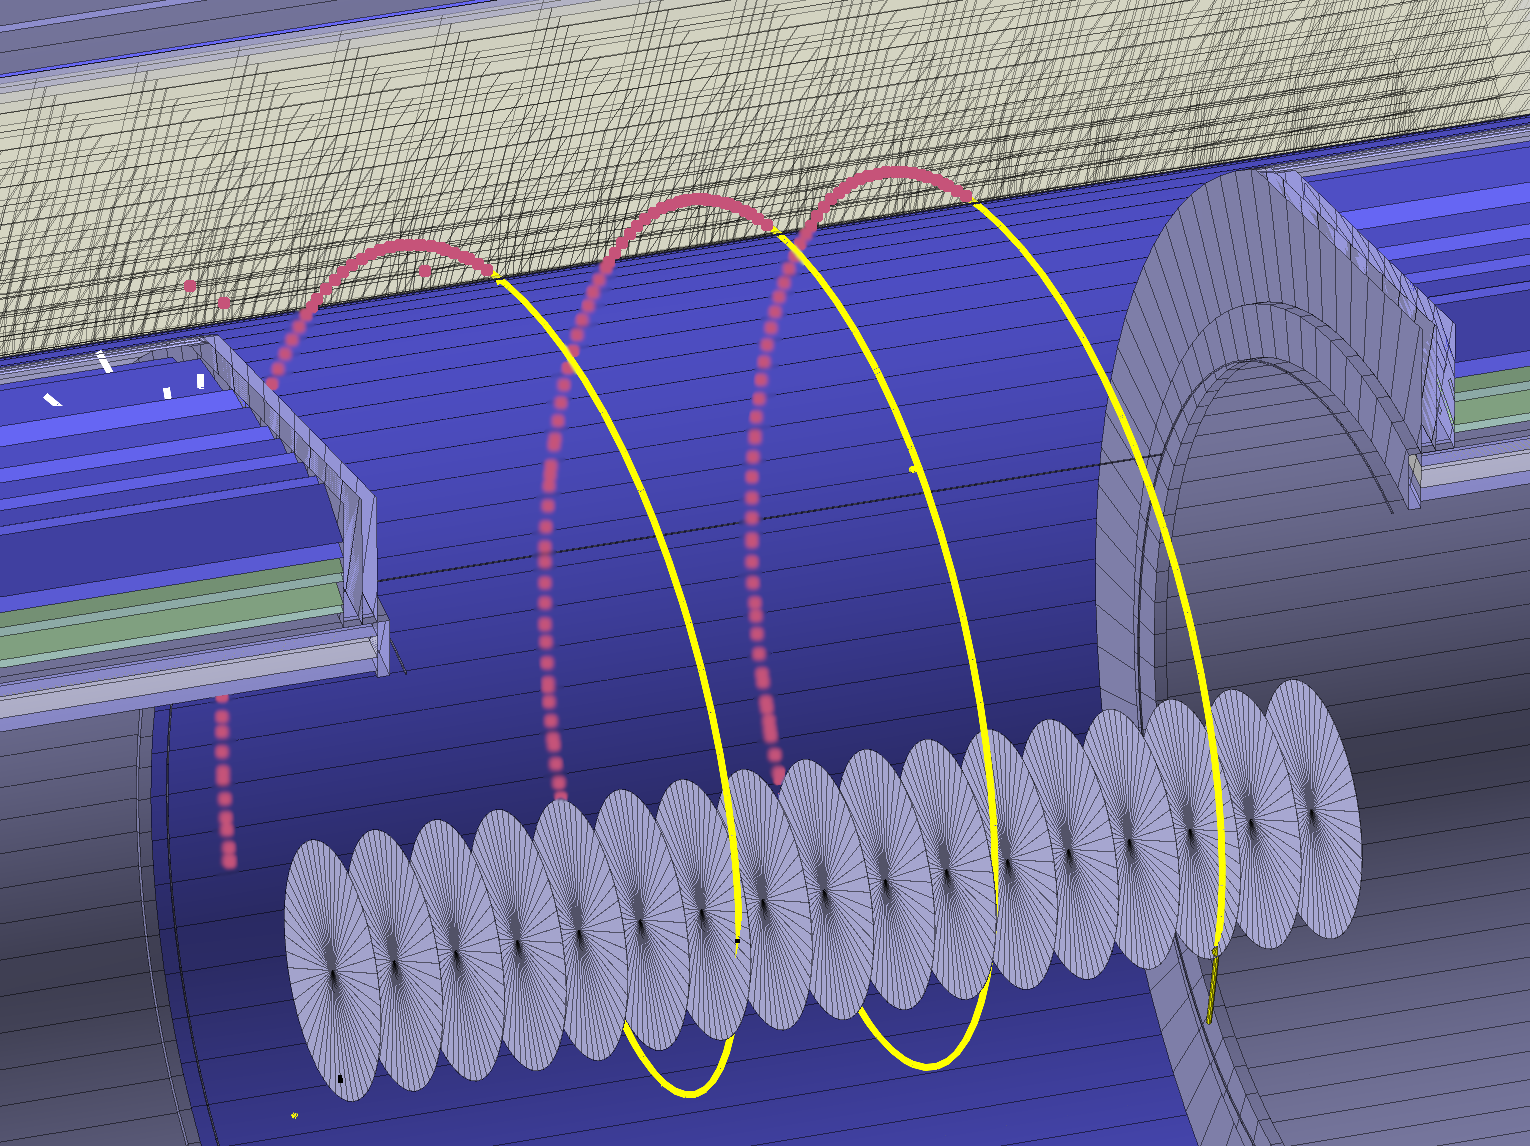
\includegraphics[width=0.5\textwidth]{chapter3/hit_instances_blur_crop.png}
    \caption{Hits, shown as red dots, produced by the CDC's sensitive detector class when a particle deposits charge inside the gas. One instance of \texttt{IG4HitGas} is created every time the particle traverses a CDC cell, i.e.\ roughly every \SI{16}{mm}.}
    \label{fig:sim_cdc_hits}
\end{figure}


This new hit class and the associated algorithms were introduced to \SimG in 2019. This hit representation is designed toward gaseous detectors, hence it also applies to the Straw-Tube Tracker of Phase-I and Phase-II. 
Because of the relatively low density of hit instances along a trajectory, important details of the true energy deposition pattern may be lost. Hence \SimG implements a run-time option to store \emph{auxiliary points} inside each hit instance, which provide a more fine-grained description of the particle's steps inside the cell.

% The \texttt{IG4HitGas} class was designed to condense and record energy loss information inside gaseous ionisation detectors in \SimG (e.g. the CDC and Straw-Tube Tracker). Every energy deposit made by a particle inside the same CDC cell is accumulated into a single instance of the class, such that only one hit per cell per particle may exist. While this saves memory and disk space, it limits the amount of detail that can be stored. The recorded information allows for basic detector response simulation, but if more detail is required one can tune the \SimG simulation to store finer details inside each \texttt{IG4HitGas} instance.



\section{Large-scale simulation: MC5}
\label{sec:mc5}
The 5th large-scale production of simulation data, MC5, was run in 2020 using computing facilities at the French National Institute of Nuclear and Particle Physics Computing Centre (CC-IN2P3) in Lyon, France.
Using \numprint{2000} concurrent machines over the course of a few weeks, the outcomes of 1 billion proton-on-target (POT) collisions were simulated with \SimG in the CyDet configuration of COMET Phase-I.

\subsubsection{Software}
Leading up to the MC5 production, several aspects of the software were changed or updated in comparison with the previous large-scale production:
\begin{itemize}
    \item The CMake build configuration system was introduced to replace the legacy CMT system. 
    \item The external ROOT software, upon which the \oaEvent data format depends, was updated from major version 5 to 6.
    \item The CyDet geometry received multiple updates to make it as faithful as possible to the design, adding detailed elements such as readout boards and fixing errors in the positioning of CDC wires. 
    \item As discussed in Section~\ref{subsec:SD}, the treatment of energy deposits in the CDC was also changed to the \texttt{IG4HitGas} representation.
    \item All memory-related problems identified by \texttt{valgrind} at the time were resolved to bring the simulation software into a production-ready state.
\end{itemize}

\subsubsection{Run configuration}

\begin{figure}
    \centering
    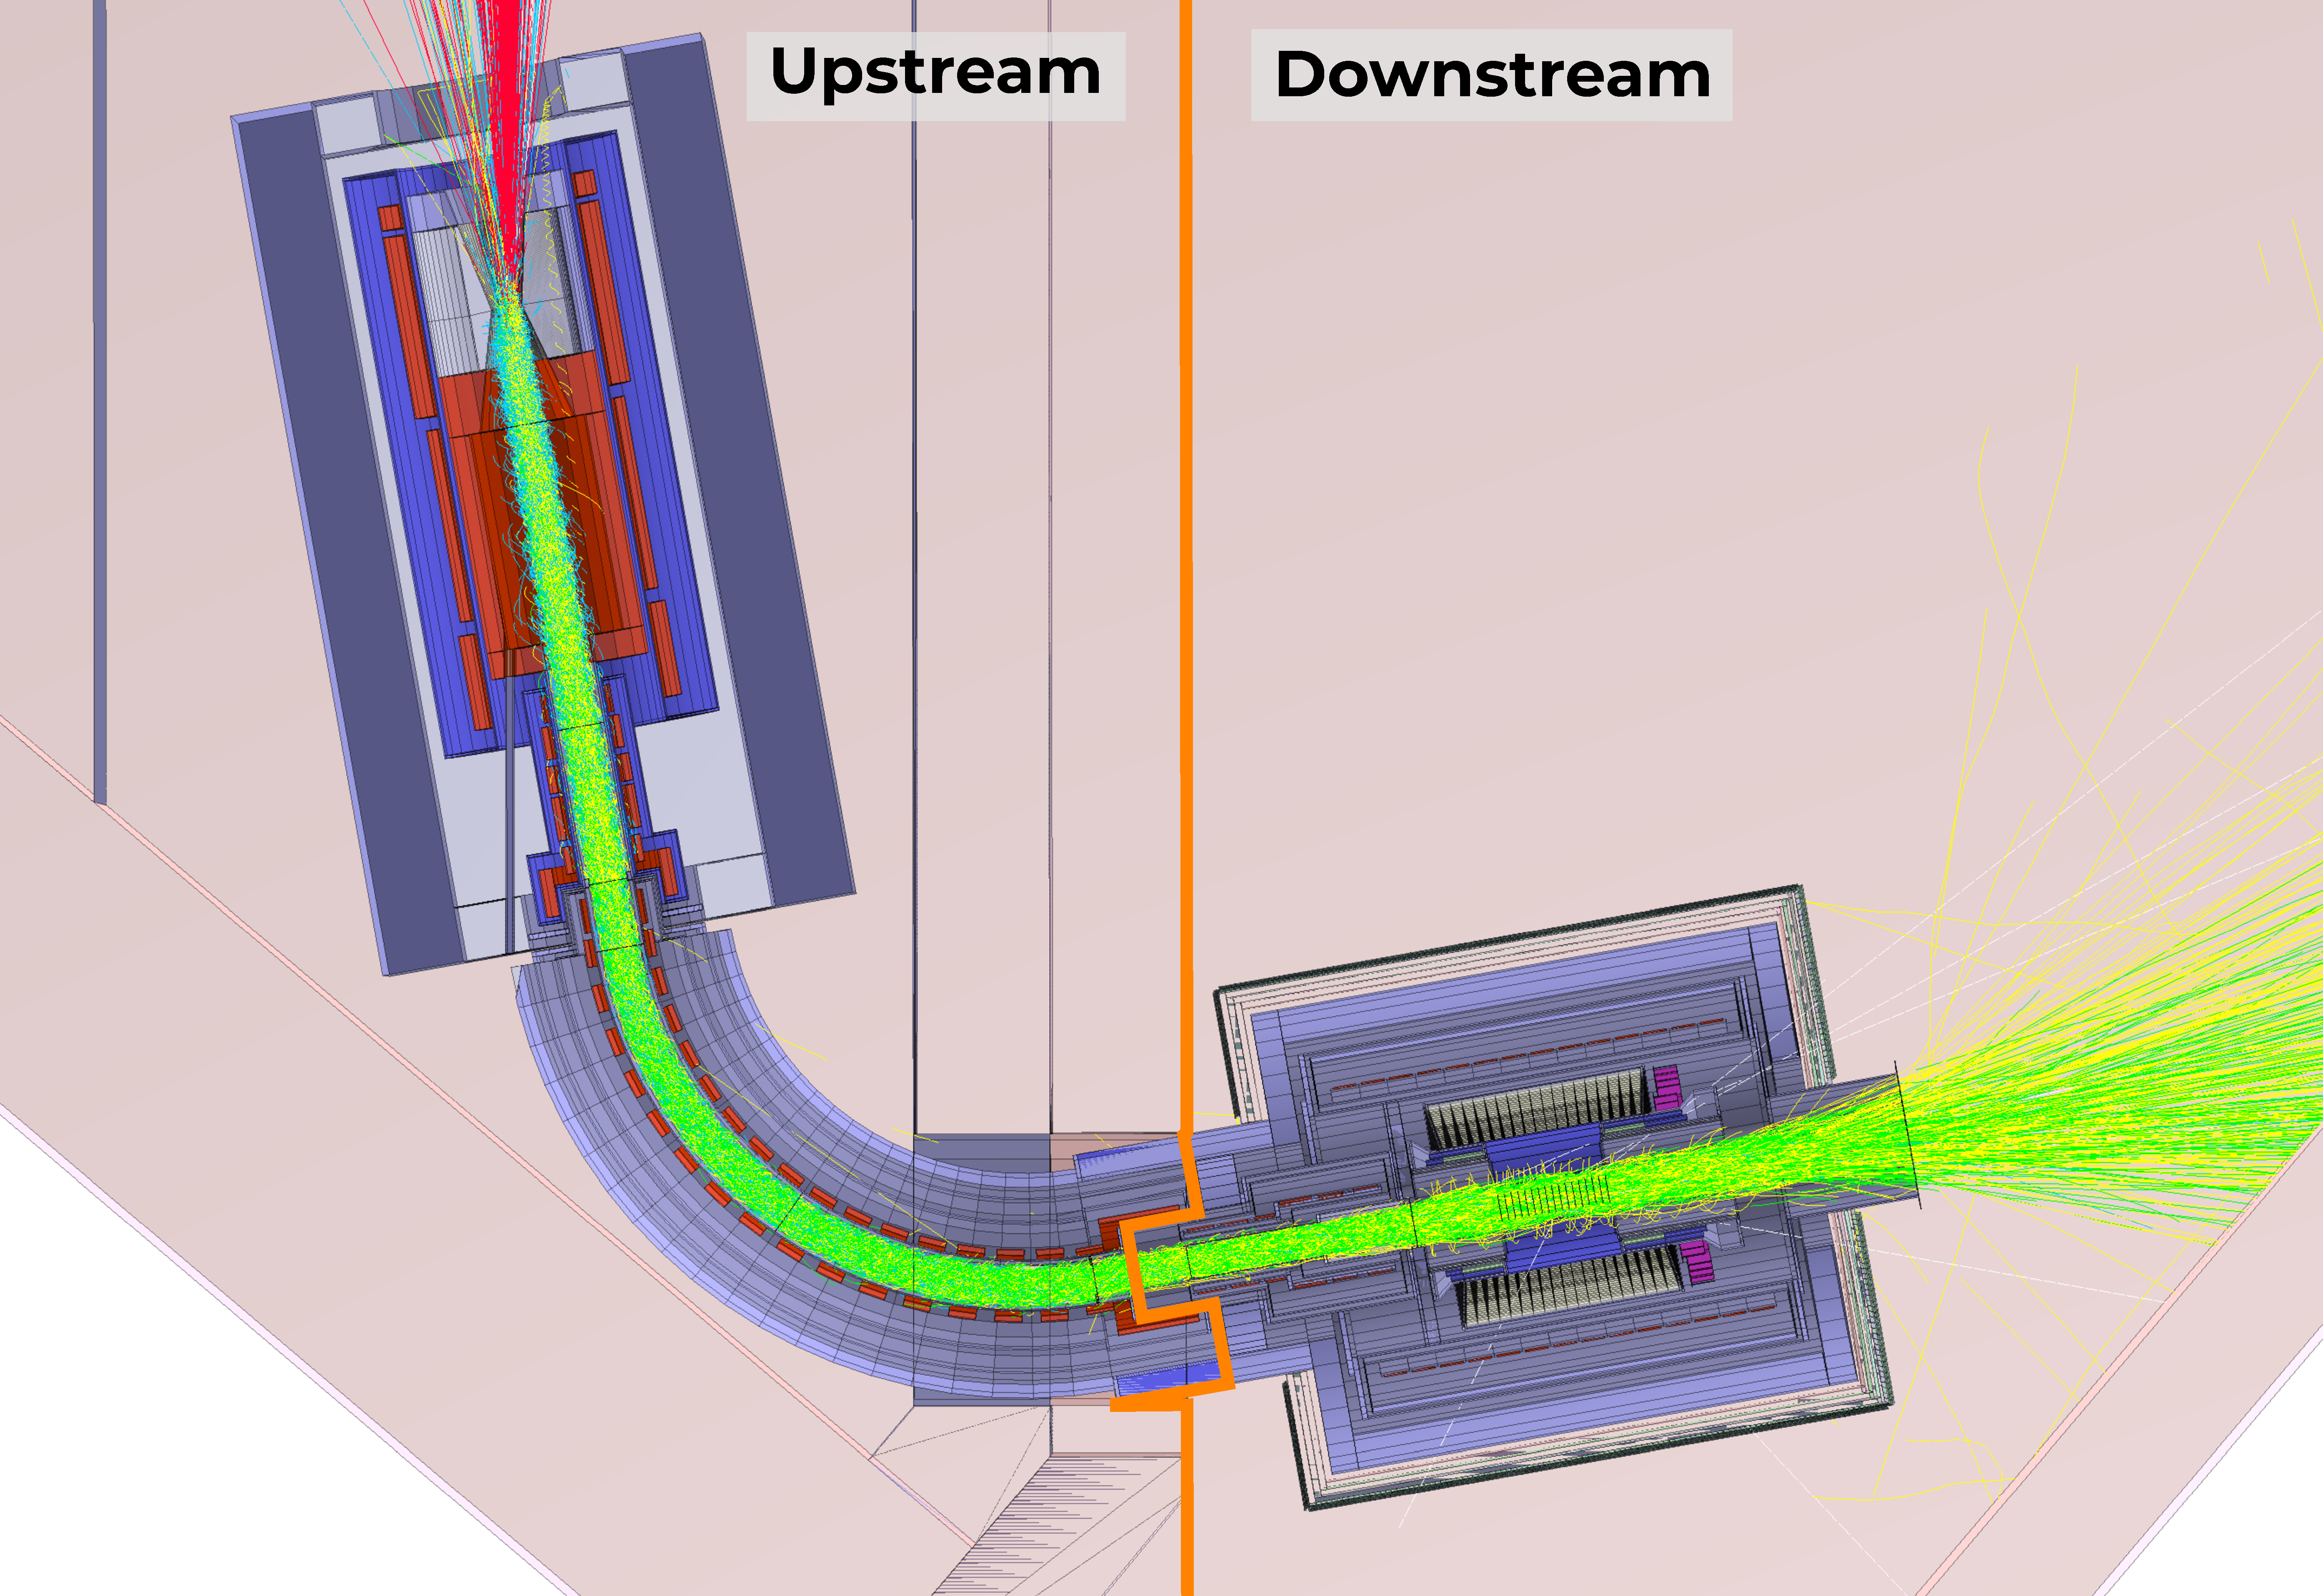
\includegraphics[width=0.6\textwidth]{chapter3/sampling_plane_illu_ink.pdf}
    \caption{
        Top-down cutaway view of the running configuration for MC5,
        showing $1.6\times 10^5$ overlaid events (1\% of a bunch). The orange
        line shows the sampling boundary where particles that cross into the
        detector region via the beamline or wall are recorded. Only
        charged-particle trajectories are shown for clarity.
    }
    \label{fig:Phase-I Sampling World}
\end{figure}



The simulation was split into two stages by dividing the world along a boundary
which effectively separates the pion-production section and transport solenoid
(upstream) from the detector region (downstream), as shown in
Figure~\ref{fig:Phase-I Sampling World}. The boundary is set up to record the
position and momentum of particles which enter the detector region. Most
particles will enter via the beamline, but a small fraction (mostly neutrons)
also penetrates through the wall, floor and ceiling. In the upstream run, only
particles that enter the detector region are saved to disk, along with their
ancestors. Upon doing so, their position and momentum is recorded to an
\texttt{oaRooTracker} file (see Section~\ref{subsec:RT}) which is used as input for the
downstream simulation.

This way to proceed means that the upstream simulation is unaffected by the disposition of the detector region, hence one can perform the upstream run once and use the results to seed multiple downstream configurations, e.g.\ changing the detector geometry (e.g.\ between CyDet and the StrawECAL) or magnetic field. Since most of the simulation time is spent in the pion-production section, this gives a flexible way to produce high-statistics MC datasets in multiple experimental configurations.
%Another benefit is that it allows for re-seeding of the downstream run, whereby each event retains the same initial conditions but uses several different seedings of the random number generator, yielding a more diverse dataset at the cost of potentially biasing the sample.
% ^ Off-topic?

\subsubsection{Outcome}
The data produced with MC5 has a total disk size of \SI{13}{TB} and is archived on the tape storage system at CC-IN2P3. The sample size of $10^9$ POT events represents 62 unique beam bunches when merged, or the equivalent of $~\SI{0.1}{\ms}$ of data acquisition in Phase-I.

\section{Animated CyDet event display}
In order to visualise events in the CyDet system, I developed a tool to display hit data from MC simulations as animations, visually similar to a slow-motion online monitor of the detector. Figure~\ref{fig:animation} shows a series of frames from one such animation involving a $\mu$--$e$ conversion electron.

\begin{figure}
    \centering
    
    \captionsetup[subfigure]{justification=centering}
    \begin{subfigure}[t]{0.49\textwidth}
    \centering
    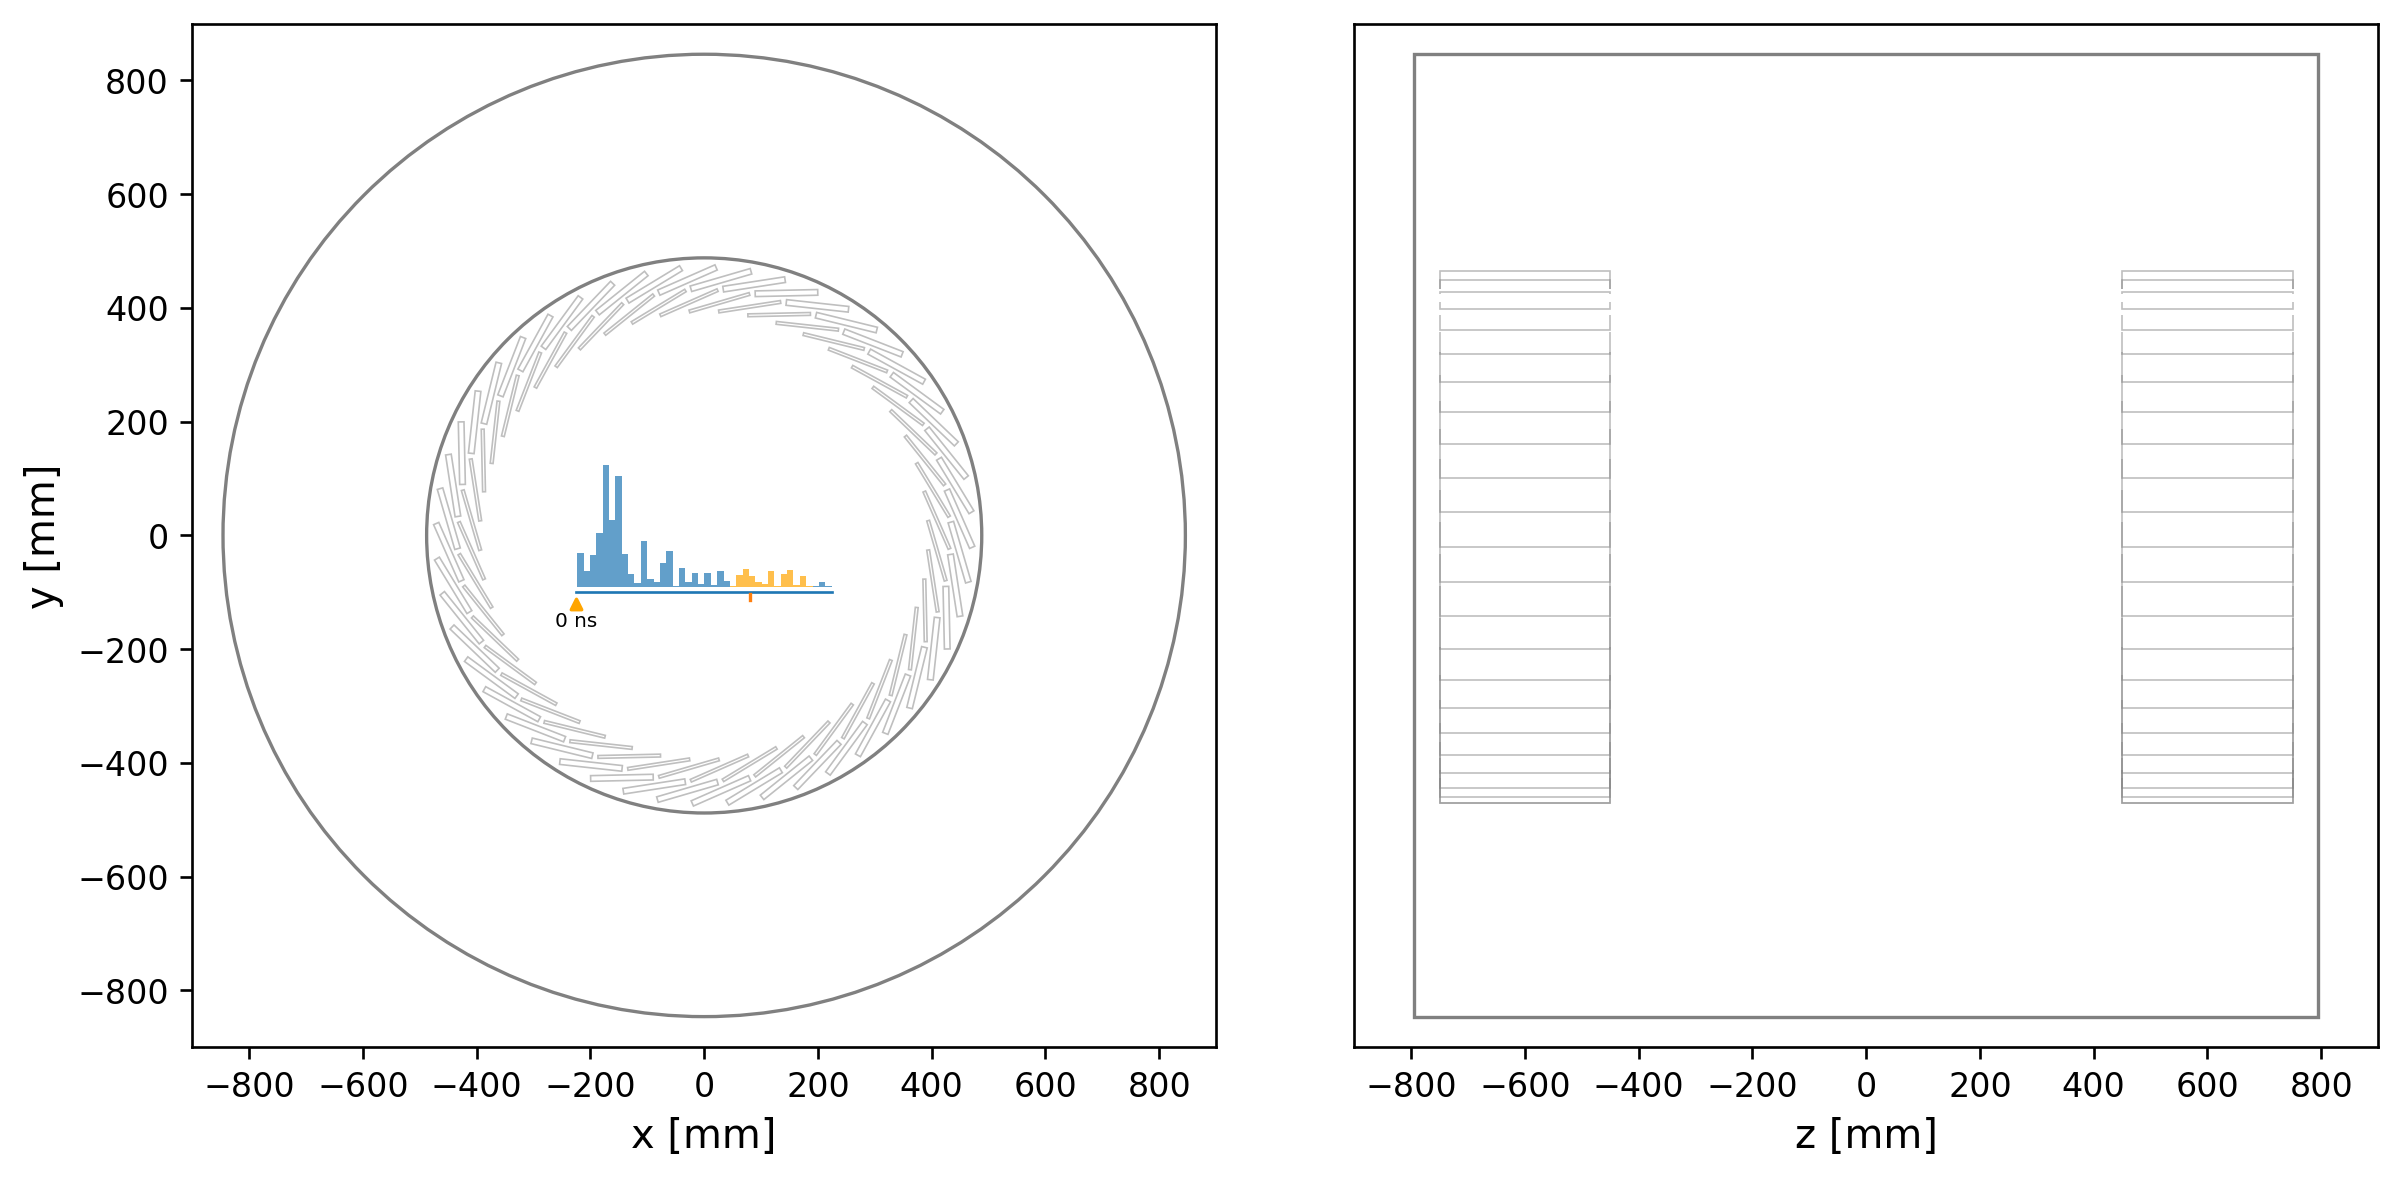
\includegraphics[width=0.95\textwidth]{chapter3/frame_005.png}
    \caption{$t=\SI{0}{ns}$. Ignoring pileup and cosmics, the detector is clear of hits before the POT collision.}
    \end{subfigure}
    \hfill
    \begin{subfigure}[t]{0.49\textwidth}
    \centering
    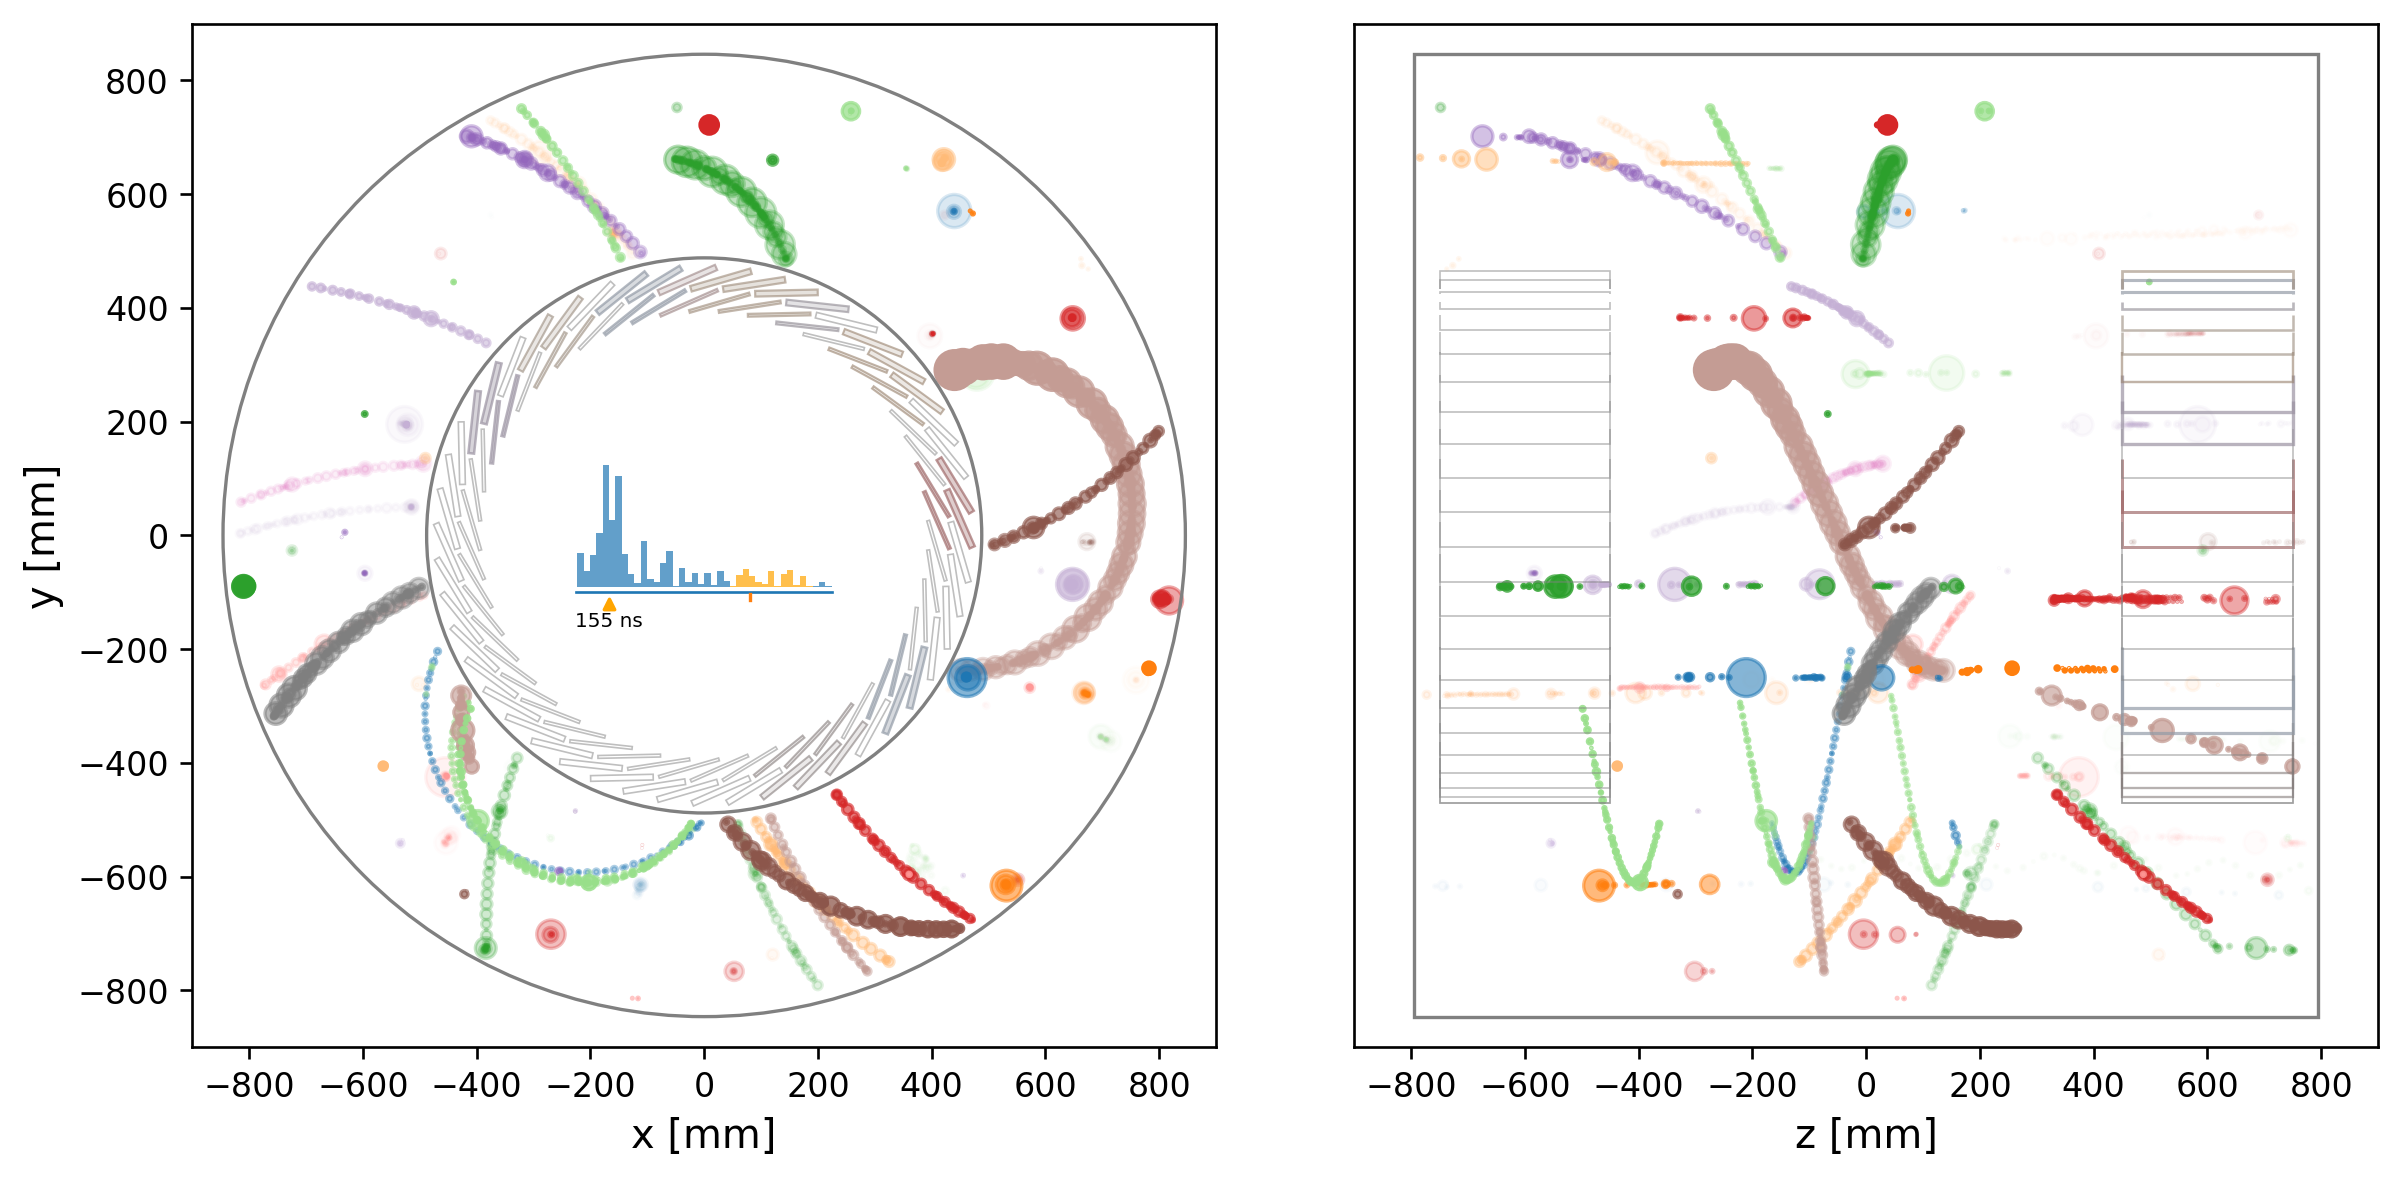
\includegraphics[width=0.95\textwidth]{chapter3/frame_036.png}  
    \caption{$t=\SI{155}{ns}$: many tracks occupy the detector soon after the beam flash.}
    \end{subfigure}
    
    \vspace{0.3cm}
    
    \begin{subfigure}[t]{0.49\textwidth}
    \centering
    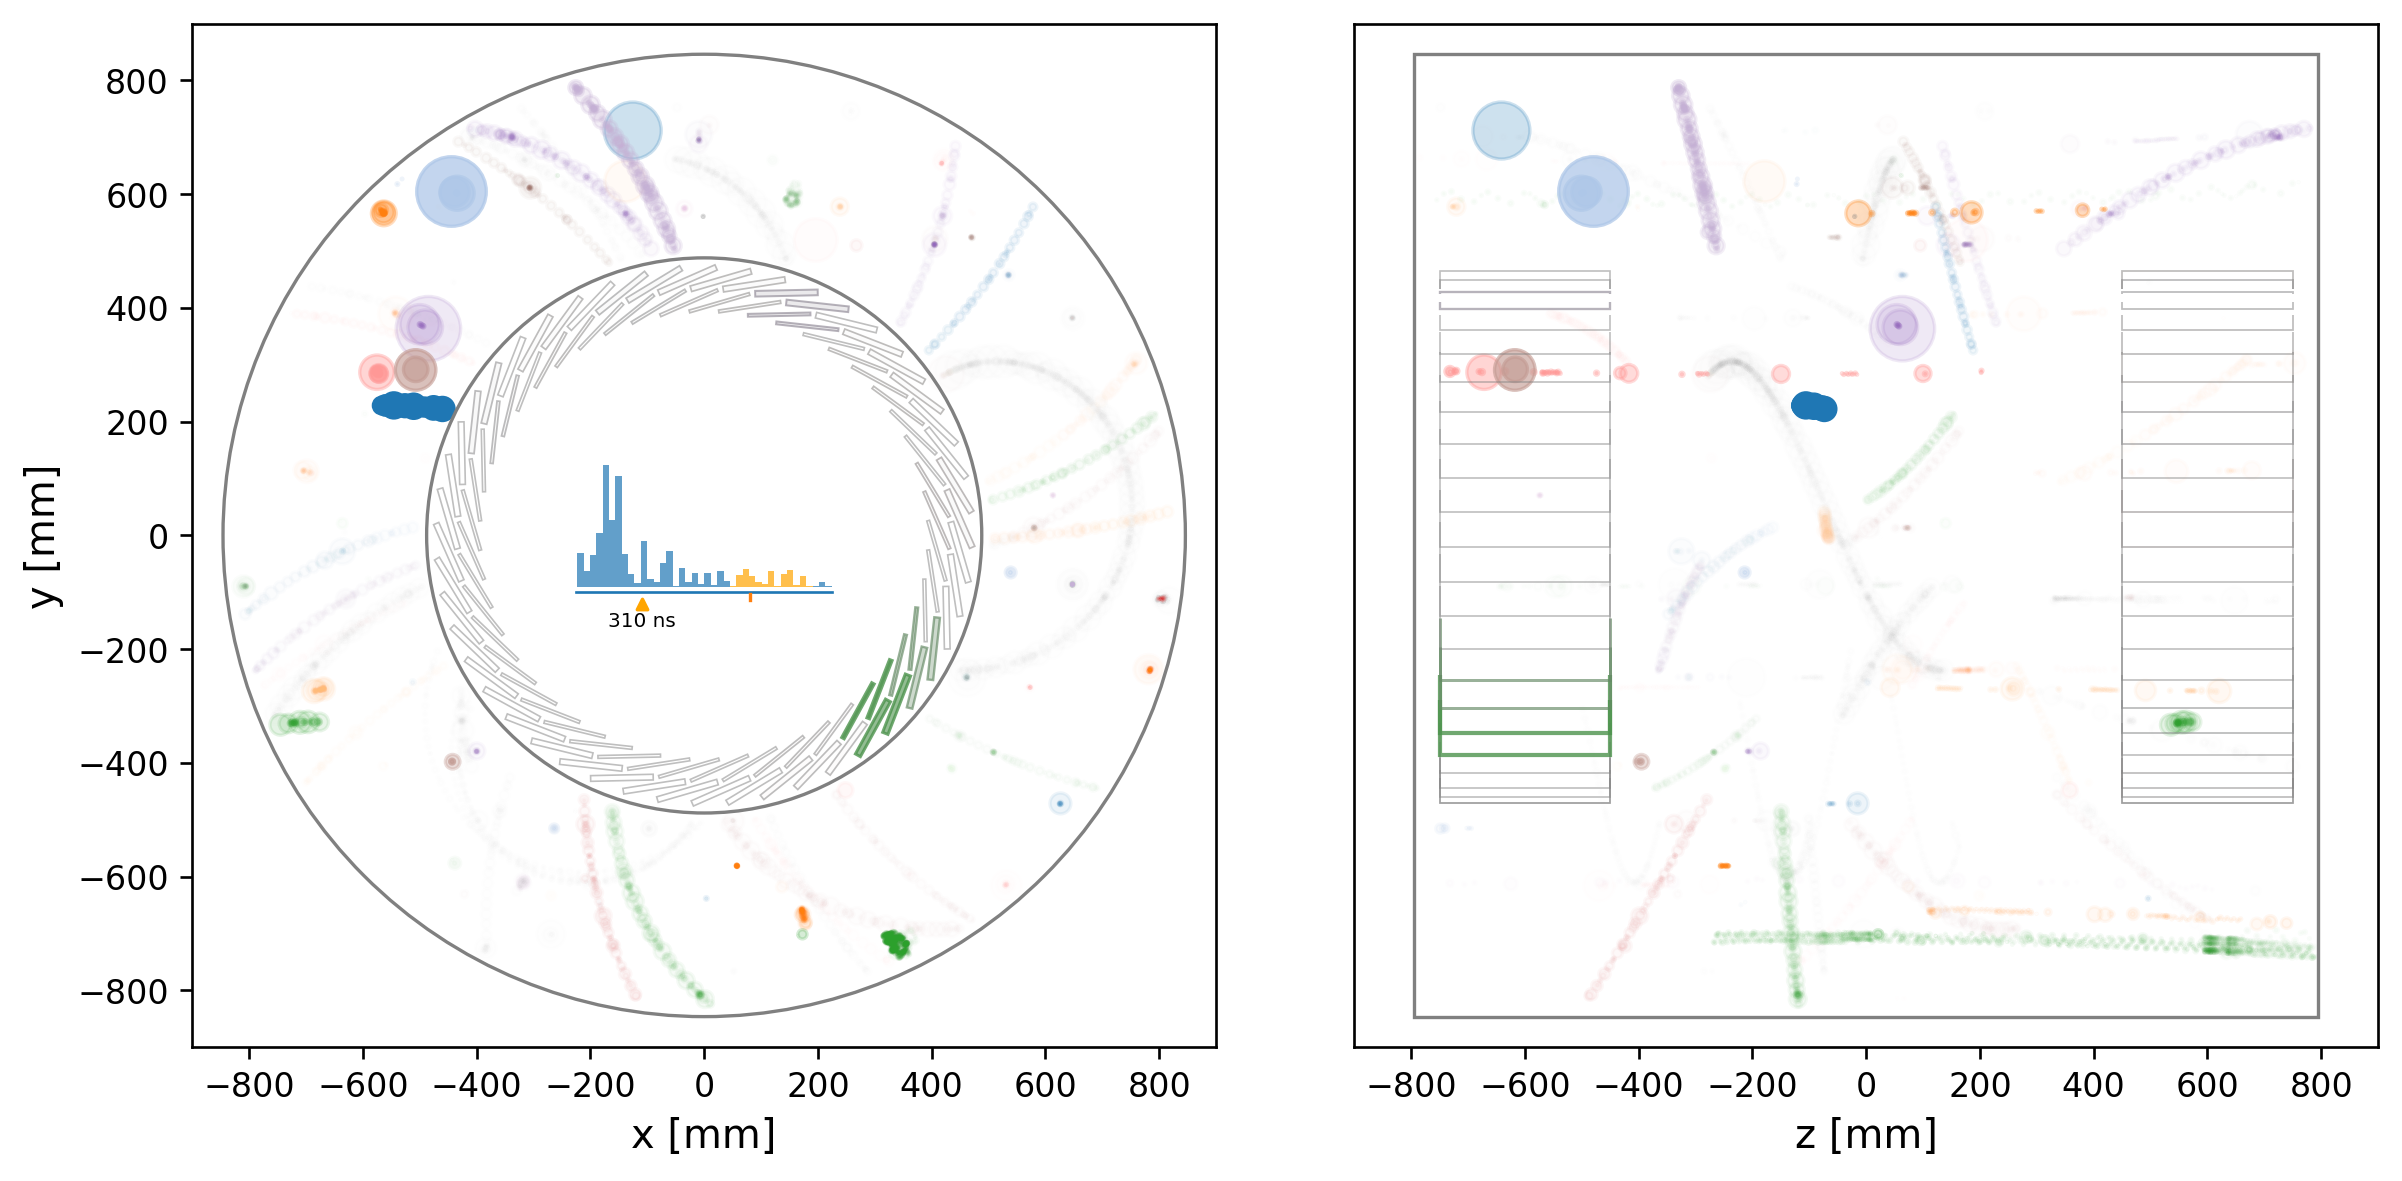
\includegraphics[width=\textwidth]{chapter3/frame_067.png}
    \caption{$t=\SI{310}{ns}$: the hit rate decreases significantly once the beam flash has ended.}
    \end{subfigure}
    \hfill
    \begin{subfigure}[t]{0.49\textwidth}
    \centering
    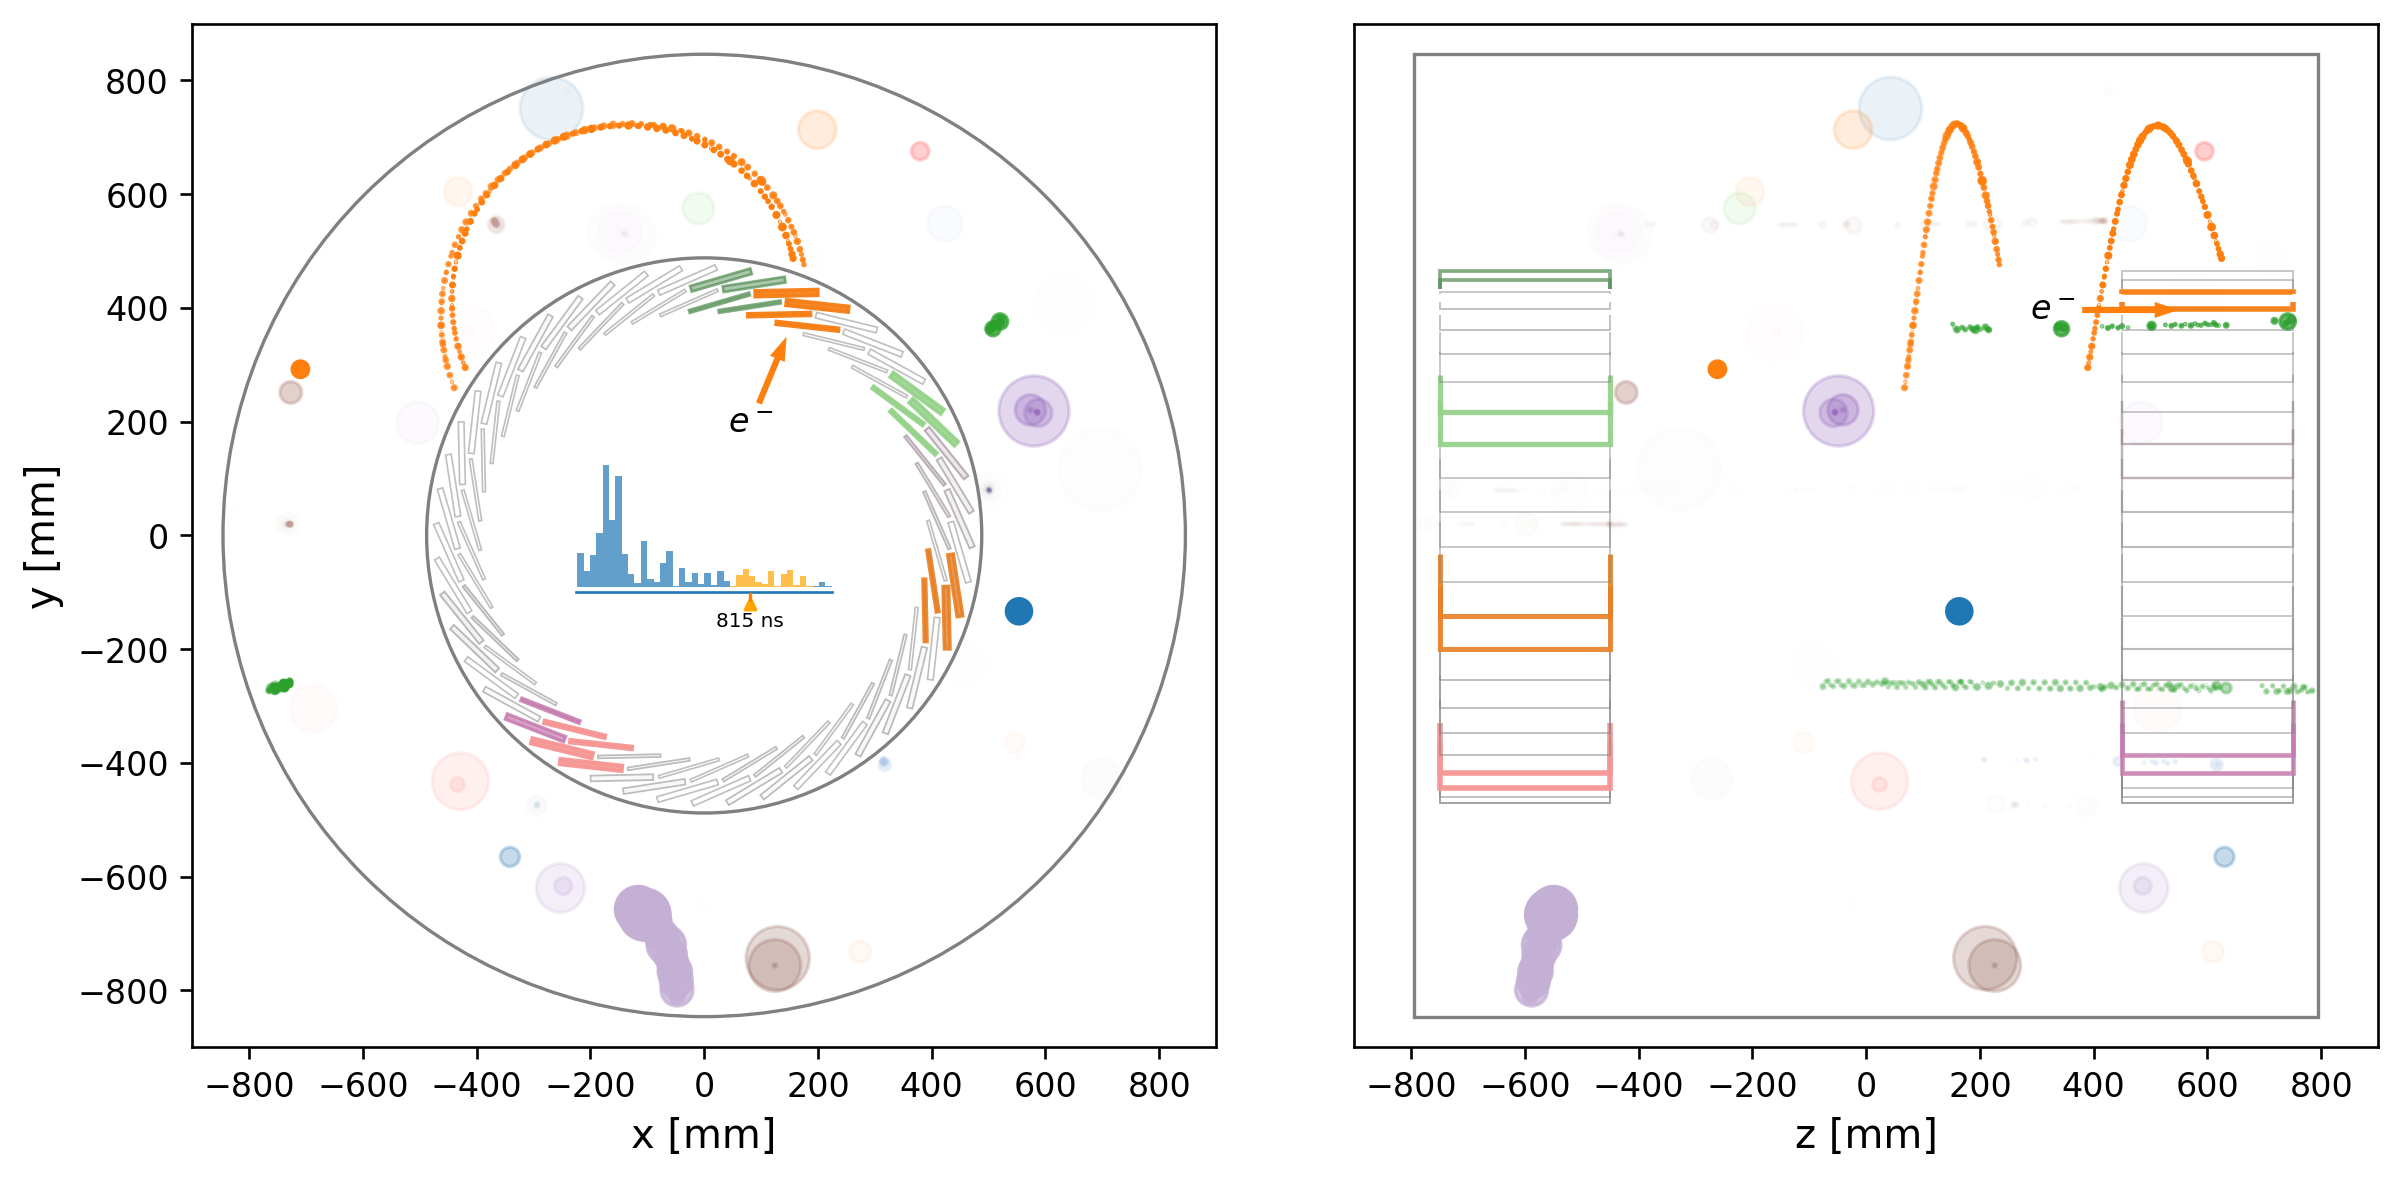
\includegraphics[width=\textwidth]{chapter3/frame_192.png}
    \caption{$t=\SI{815}{ns}$: a conversion electron appears in the CDC and triggers the CTH.}
    \label{fig:animation:conv}
    \end{subfigure}
    
    \caption{Still frames of an animation rendered by the visualisation tool. The event shown outlines how a conversion electron would be seen by the CyDet system among background hits.}
    \label{fig:animation}
\end{figure}


% Visual features
The produced animations show the CyDet system under two projections such that particle trajectories can be visualised in all three dimensions, over time. The left-hand side of the display shows the projection in the readout plane, with the CDC on the outside and the CTH counters on the inside, while the right-hand side shows an orthogonal view with the same vertical axis.
In the centre of the left-hand pane, a histogram shows the rate of hits over the event's duration and a cursor indicates the current time in the simulation.

Each animation shows one bunch event unfolding over one cycle, i.e.\ \SI{1170}{\ns} from the collision of one bunch until the arrival of the next one. Time is slowed down by a factor of ${\sim}10^{-7}$ such that the event unfolds over 10 real seconds.

In the CDC, the true position of every hit is drawn as a circle with a radius proportional to the amount of energy deposited. Colour indicates hits produced by the same particle such that tracks can be disambiguated.

The CTH counters flash only in the case of a fourfold coincidence i.e.\ if four adjacent counters are struck within a \SI{10}{\ns} window.
Fourfold coincidences are most often caused accidentally by multiple particles, but occasionally a single track will hit four counters. In these occurrences, the track is emphasised in the animation and the particle type is displayed, as can be seen in Figure~\ref{fig:animation:conv}.

Hits in the CDC and CTH fade out over time such that the display does not become cluttered, but the fading rate is not representative of the actual time resolution of the sub-detectors.

% Implementation details
The animation rendering tool is written in Python. The code includes an algorithm for finding fourfold coincidences among CTH hits. To draw the frames, it relies on the \texttt{matplotlib} package. Once the individual frames have been rendered, a \texttt{bash} script runs \texttt{ffmpeg} to assemble them into a video format, such as \texttt{webm}, \texttt{gif} or \texttt{mp4}.


\section{Version control and continuous integration}

The source code of the ICEDUST software project is version-controlled using Git. A shared repository is hosted on the Gitlab instance of the IN2P3, where developers collaborate on building up and improving the code base. The repository contains a full history of the code, an issue tracker, and a set of wiki pages documenting the software. 

Additions and changes are submitted to the central repository through merge
requests from the developers. When submitting a merge request, changes to the
code are typically reviewed by another developer or maintainer who verifies that
no new bugs are introduced into the main branch. To further reduce the
likelihood of new issues appearing, the ICEDUST repository makes use of Gitlab's
continuous integration system.

Every time new code enters the main branch, the whole code base goes through a
three-step pipeline. The first step compiles the code and builds a new version
of every binary. The second step runs custom unit tests and validations using
this new build. Each unit test typically verifies that a single functionality
works as intended in an isolated environment, while validations can run multiple
pieces of the software and ensure that the results are consistent between one
revision of ICEDUST and the next.

If the building, unit testing and validation stages all pass, the pipeline moves to the final deployment step where the new binaries are assembled into a Docker image which is published to the repository's container registry. Users who wish to use the compiled software as-is can download this image and run it via Docker or Singularity.
If any of the pipeline steps reports a failure, the developer submitting the merge request is notified and full logs are provided to identify the issue. A merge request is usually only accepted once the code has been reviewed and if the pipeline finishes successfully.

